%% This file is modified by Veli Mäkinen from HY_fysiikka_LuKtemplate.tex authored by Roope Halonen ja Tomi Vainio.
%% Some text is also inherited from engl_malli.tex by Kutvonen, Erkiö, Mäkelä, Verkamo, Kurhila, and Nykänen.


% STEP 1: Choose oneside or twoside
\documentclass[english,twoside,openright]{HYgraduMLDS}
%finnish,swedish

%\usepackage[utf8]{inputenc} % For UTF8 support. Use UTF8 when saving your file.
\usepackage{lmodern} % Font package
\usepackage{textcomp} % Package for special symbols
\usepackage[pdftex]{color, graphicx} % For pdf output and jpg/png graphics
\usepackage[pdftex, plainpages=false]{hyperref} % For hyperlinks and pdf metadata
\usepackage{fancyhdr} % For nicer page headers
\usepackage{tikz} % For making vector graphics (hard to learn but powerful)
%\usepackage{wrapfig} % For nice text-wrapping figures (use at own discretion)
\usepackage{amsmath, amssymb} % For better math
\usepackage{listings} % For long ass verbatims
\usepackage{cite} % For ordered citations
\usepackage{algorithm} % For better pseudocode algorithms
\usepackage{algpseudocode} % The same as previous
%\usepackage{csquotes} % Block quotes
\usepackage [autostyle, english = american]{csquotes}
\MakeOuterQuote{"}

\lstset{
basicstyle=\small\ttfamily,
columns=flexible,
breaklines=true
}
%\usepackage[square]{natbib} % For bibliography
\usepackage[footnotesize,bf]{caption} % For more control over figure captions
\usepackage{blindtext}
\usepackage{titlesec}
\usepackage[titletoc]{appendix}

\onehalfspacing %line spacing
%\singlespacing
%\doublespacing

%\fussy 
\sloppy % sloppy and fussy commands can be used to avoid overlong text lines

% STEP 2:
% Set up all the information for the title page and the abstract form.
% Replace parameters with your information.
\title{Clustering of programming exercises for efficient reviewing and exploration}
\author{Teemu Koivisto}
\date{\today}
\prof{Dr. Arto Hellas}
\censors{Professor Jussi Kangasharju}{}{}
\keywords{programming education, MOOCs, clustering, similarity detection, ASTs, CodeClusters}
\depositeplace{}
\additionalinformation{}


\classification{
\\
Computing methodologies $\rightarrow$  Machine learning $\rightarrow$  Learning paradigms $\rightarrow$  Unsupervised learning \\
Information systems $\rightarrow$  Information retrieval $\rightarrow$  Retrieval tasks and goals $\rightarrow$ Clustering and classification\\
Information systems $\rightarrow$  Information systems applications $\rightarrow$  Data mining\\
Social and professional topics $\rightarrow$  Professional topics $\rightarrow$  Computing education $\rightarrow$  Computing education programs $\rightarrow$ Computer science education}

% if you want to quote someone special. You can comment this line and there will be nothing on the document.
%\quoting{Bachelor's degrees make pretty good placemats if you get them laminated.}{Jeph Jacques} 


% OPTIONAL STEP: Set up properties and metadata for the pdf file that pdfLaTeX makes.
% But you don't really need to do this unless you want to.
\hypersetup{
    bookmarks=true,         % show bookmarks bar first?
    unicode=true,           % to show non-Latin characters in Acrobat’s bookmarks
    pdftoolbar=true,        % show Acrobat’s toolbar?
    pdfmenubar=true,        % show Acrobat’s menu?
    pdffitwindow=false,     % window fit to page when opened
    pdfstartview={FitH},    % fits the width of the page to the window
    pdftitle={},            % title
    pdfauthor={},           % author
    pdfsubject={},          % subject of the document
    pdfcreator={},          % creator of the document
    pdfproducer={pdfLaTeX}, % producer of the document
    pdfkeywords={something} {something else}, % list of keywords for
    pdfnewwindow=true,      % links in new window
    colorlinks=true,        % false: boxed links; true: colored links
    linkcolor=black,        % color of internal links
    citecolor=black,        % color of links to bibliography
    filecolor=magenta,      % color of file links
    urlcolor=cyan           % color of external links
}

\begin{document}

% Generate title page.
\maketitle

% STEP 3:
% Write your abstract (of course you really do this last).
% You can make several abstract pages (if you want it in different languages),
% but you should also then redefine some of the above parameters in the proper
% language as well, in between the abstract definitions.

\begin{abstract}
Programming courses often receive large quantities of program code submissions to exercises which, due to their large number, are graded and students provided feedback automatically. Teachers might never review these submissions therefore losing a valuable source of insight into student programming patterns.

This thesis researches how these submissions could be reviewed efficiently using a software system, and a prototype, CodeClusters, was developed as an additional contribution of this thesis. CodeClusters' design goals are to allow the exploration of the submissions and specifically finding higher-level patterns that could be used to provide feedback to students. Its main features are full-text search and n-grams similarity detection model that can be used to cluster the submissions.

Design science research is applied to evaluate CodeClusters' design and to guide the next iteration of the artifact and qualitative analysis, namely thematic synthesis, to evaluate the problem context as well as the ideas of using software for reviewing and providing clustered feedback. The used study method was interviews conducted with teachers who had experience teaching programming courses.

Teachers were intrigued by the ability to review submitted student code and to provide more tailored feedback to students. The system, while still a prototype, is considered worthwhile to experiment on programming courses. A tool for analyzing and exploring submissions seems important to enable teachers to better understand how students have solved the exercises. Providing additional feedback can be beneficial to students, yet the feedback should be valuable and the students incentivized to read it.

\end{abstract}

% Place ToC
\mytableofcontents

\mynomenclature

\chapter{Introduction}
\label{ch:introduction}
Thousands of programming courses use programming exercises as part of their curriculum. It is widely accepted that hands-on exercises help students to understand and learn concepts more deeply than without them. A crucial part of exercises is grading them, so that the students can confirm they have correctly understood a given concept. Another important part is providing feedback to students, to guide them to improve their work to better match the requirements for a given exercise \cite{survey-feedback-gen, doing-feedback-well, towards-providing-feedback}.

On these assumptions, it is then highly desirable to grade the exercises students have submitted and to provide feedback to students. The most primitive approach would be to manually grade all of the student submissions and to provide individual feedback to every student. This, however, faces the limits of the teacher's capability to review code. It is not uncommon for a course to receive hundreds or even thousands of submissions each week \cite{overcode, codewebs, stanford-million, fox-clust-leverage-2015}. Even with the help of multiple teaching assistants, the scale of the problem is considerable and the reviewing often monotonous.

A common solution to this problem is to use automated tests \cite{tmc, automatic-tests, aalto-2010-auto-ass-systems-review, aalto-2001-auto-asses, alamutka-2005-auto-ass-survey}. For every exercise, teacher would create a set of tests that would validate the submission on a series of test inputs and output the results of each test. These results would then be sent to the students who could then use it as feedback to improve their code. The passed and failed tests could be quantified into a single numeric value as the test score. With this type of system, it eliminates the need for teachers to manually review and grade the exercises. Automatic grading could also be more consistent due to the objectivity of tests, faster and have around the clock availability \cite{ala-mutka-2003-caa-review, alamutka-2005-auto-ass-survey}. After creating the proper test-suites and pipeline, the time required to manage the system would become minimal \cite{auto-ass-tools-2017, alamutka-2005-auto-ass-survey}.

\iffalse
alamutka2005
Teachers often agree that it is not possible to assess automatically all the issues relating to good programming.

With larger assignments, a more common approach seems to be to combine manual and automatic assessment.
\fi

This solution, however, involves a trade-off. While the automated tests would remove the need for teachers to manually assess the code, they could stop reviewing the submissions all together. They would then have to trust the tests to capture all the possible variations of incorrectness and this also might lead to teachers becoming unsure about the programming patterns of their students and force them to rely on the test scores to indicate any gaps in the students' understanding.

Of course, in most cases, teachers would have other ways to analyze their students' behavior. If student assistance chat channels, forums or lab sessions exist, teachers could use them to gauge student misconceptions and problems \cite{multi-faceted-mooc-support, glassman-reusable-feedback}. Having the historical data on attempted submits showing each failed test would be helpful in knowing what problems the students have struggled the most with \cite{glassman-reusable-feedback}. In some cases, there are even tools in use that show snapshots of students' code to display their progress towards solving an exercise \cite{snapshots}. Still, none of these approaches provide a synthesis of the higher-level patterns of the student code.

It has been suggested that when the exercises are automatically assessed some students might start to optimize their effort to do only the bare minimum to pass them, disregarding quality aspects \cite{aalto-2010-auto-ass-systems-review}. It might also tempt the students to attempt tricking the automatic grading system \cite{alamutka-2005-auto-ass-survey}. Hence, if the students knew that their code would be reviewed by the teacher, it might incentivize them to better uphold the quality of their code as well as to discourage the students from bypassing the tests. Perhaps even plagiarism would decrease with greater teacher oversight.

Other ways to grade the exercises exist that would eliminate the need for the teachers to review code, such as self-grading or peer grading, yet they have not been proven as reliable as teacher-authored grading \cite{self-peer-grading, codewebs, divide-and-correct}. If we expected teachers to be able to access the code and review it, they would still have to face the same problem as with the manual reviewing - there are too many submissions to go through one by one \cite{overcode, codewebs}.

The problem of analyzing a large set of documents to find interesting patterns and to provide feedback, could be labelled as an information retrieval problem. Information retrieval (IR) is a vast topic entailing the fundamentals of finding the most relevant information out of a large dataset, as well as how it could be built into a software system \cite{ir-in-practise, intro-to-ir}. Google Search\footnote{\url{https://www.google.com/}} is perhaps the most ubiquitous IR system, which proves that the search engine is a versatile and robust tool for searching huge datasets. Search engines have also been applied to the searching of code from git repositories\footnote{\url{https://github.com/search}} but would it be possible to apply it for student code submissions? More importantly, would it even solve the problems teachers face?

If we thought the search engine as a simple full-text search, the teachers could find various data structures, libraries or patterns with pattern-based matching. They could be then used as indicators for possible misconceptions or distinct structural patterns. However, to resolve all their reviewing with text searches would be impractical, as inventing new search queries would be time-consuming and their use for discerning higher-level structural patterns unreliable. Instead, a much faster approach could be to find the similar patterns automatically and letting teachers review them as groups. This could immediately visualize the variations between the submissions without burdening the teachers with extensive manual review. The similarity could be based on the solution schemas students have used to solve the exercises which are defined by their distinct use of tokens and control-flow, or using other, smaller patterns\cite{overcode}. Additionally, teachers could be interested in finding the submissions that are very far apart from the rest - the outliers.

Systems have been proposed over the years to solve this problem by reducing the dimensionality of the data to allow teachers to manage the submissions as groups instead of singular submissions. A custom search engine, Codewebs \cite{codewebs}, was developed by Nguyen et al. to enable teachers to quickly search and explore the submissions and to provide feedback based on the Abstract Syntax Trees (ASTs) of the submitted code. OverCode by Glassman et al.~\cite{overcode} is a student code reviewing and clustering system that uses unique "stack" data structures to divide the submissions into clusters. For natural language submissions, Divide and Correct by Brooks et al.~\cite{divide-and-correct} is a system to grade and provide feedback to student submissions in MOOCs using a predefined number of clusters and subclusters to keep them within manageable limits. These systems are discussed in more detail in the Section~\ref{sec:related-systems}.

Curiously, none of the systems have seen much development since their creation. Why that is can be speculated about, but this would indicate that there exists a need for this type of system. Being able to review and provide force-multiplied feedback to a large number of student submissions quickly, were there automated tests or not, could be very useful if it would not overburden the teachers with too much work \cite{aalto-2010-auto-ass-systems-review}. This is also relevant to natural language submissions, and various methods to automatize their grading and providing feedback have been researched \cite{auto-essay-scoring-case-studies, arxiv-auto-essay-grading-feedback-2018 ,divide-and-correct}. Outside the educational context, commercial services have been built that offer automated code review as a service that are somewhat similar\footnote{\url{https://aws.amazon.com/codeguru/}}. The clustering of program code in general is a quite large topic, but most of its applications have been focused on the detection of plagiarism and clones and not for educational purposes.

This thesis examines the basics of constructing a system to review and cluster student code with an ability to provide force-multiplied feedback to the students. The main question it aims to answer is: "How a system could be built to efficiently explore, analyze and provide feedback to student code submissions in programming courses?" Because this topic is very large, it is divided into four research questions:

\addtolength\leftmargini{6pt}
\begin{itemize}
    \item[\textbf{RQ1:}] How code can be represented for efficient search and modeling?
    \item[\textbf{RQ2:}] What methods can be used to analyze and cluster code?
    \item[\textbf{RQ3:}] How code submissions can be reviewed and explored efficiently?
    \item[\textbf{RQ4:}] What are the main benefits and drawbacks using CodeClusters for reviewing and exploring code?
\end{itemize}

The methods to answer them include a literature review of the fields of clustering, analysis, information retrieval, similarity detection as well as representations of code. They were chosen based on the connections drawn from the related systems as well as from having researched these topics in-depth. As an additional contribution this thesis presents a new system, CodeClusters, that implements some of these ideas and methods in practice. Exploratory design science research (DSR) analysis is applied to assess its usability and user interface (UI), and the results are used to validate its design as well as to guide the next iteration of the artifact. Also, we evaluate the problem context of teachers not being able to review the large quantities of submissions in programming courses, and the applicability of reviewing code using full-text search and n-grams based model.

As the study method, we conduct a series of interviews with teachers who have taught programming courses. Based on the interview recordings, transcripts and questionnaire answers, a thematic synthesis is carried out of the results of the interviews to find the main topics. Additionally, UI and system design criteria are used to evaluate the artifact. Then, they are used in conjunction with the literature review, the experiences developing the system and the reviewing of related systems, to answer the research questions. The goals of this thesis are to validate the problem context, the applicability of search, similarity detection and clustering for discerning patterns from submissions as well as the usability of CodeClusters.

This thesis was written as part of Data Science Master's programme at the University of Helsinki, but the software was developed for Aalto University's LeTech research group and open-sourced under the permissive MIT license \footnote{\url{https://github.com/Aalto-LeTech/CodeClusters}} \footnote{\url{https://github.com/Aalto-LeTech/CodeClustersModeling}}.

The next chapter conducts a literature review into the research fields that intersect with our topic. In Chapter~\ref{ch:system-description}, the proposed system CodeClusters is described and also a few of the related systems are reviewed. In Chapter~\ref{ch:methodology}, the research design and the structure of the interviews are described, with Chapter \ref{ch:results} and Chapter \ref{ch:discussion} containing the results and their discussion. In Chapter~\ref{ch:conclusions}, conclusions are drawn of the overall results of this thesis and its implications.


\chapter{Background}
\label{ch:background}
This background chapter presents a literature review of the different fields that intertwine with the topic of reviewing student submitted code using programmatic methods. The fields were chosen based on the research of related systems and approaches to the problem, some of them described in the Section \ref{sec:related-systems}. When taken out of the educational context, the problem could be framed as how to analyze collections of code and reduce their dimensionality to better understand and show their higher-level patterns. As such, the topic becomes quite large. Analysis of program code itself has been a research area from the early days of computing \cite{halstead-1972, mccabe-1976, ottenstein} with topics such as code quality, optimization and clone detection being quite popular \cite{chaiyong-2018}.

What makes it different for our educational setting of reviewing code, is the analysis of a large number of relatively short excerpts of code that all attempt to solve the same problem. Therefore, we can assume the dataset to be fairly homogeneous although within even a small exercise, the variation between the different approaches can become quite large \cite{luxton-sub-variation-2013}. A custom search engine that would automatically index the code in a compact, AST derived form with selectable algorithms to calculate the similarity could be a possible approach, as demonstrated by Codewebs \cite{codewebs}.

However, in order to build a similar system from scratch we have to understand the different parts that make up such system. One part, for example, would be knowing the available data structures to represent code. Knowing how to apply information retrieval to code would be useful for a good theoretical foundation. The manual reviewing process would be interesting to investigate, since it might help to understand how the process could be automated, as well as the current automatic reviewing approaches. Assuming that teachers would want to divide the submissions into groups based on their similarities, the available similarity detection and clustering methods would be important to review.

As it follows, these topics sum up to a large background research. As part of this research some of the methods are implemented in the new system, CodeClusters, which should demonstrate better their applicabilities. Being able to pragmatically test the approaches should provide more realistic depictions of the usability of the methods. However, this thesis is limited in its scope to trial all the proposed methods and therefore the approaches are picked based on the time required to implement them, their demonstrated results as well as flexibility. This thesis does not attempt to be a conclusive research into the optimal solution and system to this problem, but an analysis into the basics of building one.

In Section~\ref{sec:ir}, the ideas of the general information retrieval system, the search engine, are introduced and the most relevant concepts and methods that could be used for educational code search. In Section~\ref{sec:analyzing-code}, the manual reviewing process of the teachers is analyzed as well as the current automatic reviewing approaches. In Section~\ref{sec:representations}, the different representations of code are described. In Section~\ref{sec:metrics}, a short overview of quantification of code into numeric representations, metrics, is described. In Section~\ref{sec:sim-detection}, a few of the methods to calculate similarities between the submissions are presented. Lastly, in Section~\ref{sec:clustering}, the most common clustering algorithms are described and their applicability to our problem discussed.


\section{Information retrieval}
\label{sec:ir}
One of the earliest and most comprehensive definitions of information retrieval (IR) is by Salton (1968)~\cite{salton-1968}, which describes IR to be a field encompassing the structure, analysis, organization, storage, searching and retrieval of information. It has been primarily focused on large-scale unstructured textual data, such as web pages, but it could involve any type of data \cite{ir-in-practise}. Programming language code is considered as unstructured data although, in comparison to text or web pages, it has very formal grammar and the tokens it allows are very limited.

In our case we are interested in finding the most relevant student submissions given teacher's information need but translating these needs into particular information retrieval objectives is tricky. Our assumption is that the two most important ones are to find outliers from the dataset and also to divide it into structurally distinctive clusters. Still, these goals are not specific enough to exactly model the actual retrieval process from the user interface all the way to the used data format.

As a general description of an IR process, a user has an information need which they try to describe using a search interface of an IR system. The system executes the user's search query and returns the most relevant documents which would satisfy that need. For our educational search, the process could utilize various data as part of the retrieval, such as the number of attempted tests or the historical performance of the student, yet to simplify the scope of the research we shall only consider submitted code which has passed the tests and therefore is assumed to be correct.

Next, the most common IR system, the search engine, is described and the different IR representation models it could use. Set-theoretic models are the most simplistic models that filter the documents by marking them either \texttt{true} or \texttt{false} given search query without ranking the documents by their relevancy scores. Algebraic models allow the ranking of the documents but they are constrained to the specific ranking algorithm they use. Probabilistic models offer a more flexible approach to model the uncertainty of relevancy in their scoring but which might result in more complicated and slower models \cite{intro-to-ir, ir-in-practise}.

As this thesis does not aim to research how to construct a custom search engine for code, the research of the IR techniques is left to a general overview. The focus of the research is aimed towards the algebraic vector space model as it is a flexible method that can also be used for other purposes, and which CodeClusters uses for its similarity detection n-gram model. The main takeaways from choosing an IR model is that regardless of the model, a good weighting and similarity scoring mechanism is crucial for producing the most relevant results. A poor weighting and similarity measure will not be able to distinguish between documents of varying size and content. The possible formats to represent program code are described in more detail in the Section~\ref{sec:representations} and the similarity scoring in the Section~\ref{sec:sim-detection}. This Section was mostly based on the books \textit{Information Retrieval in Practice} (2011) by Croft et al.~\cite{ir-in-practise} and \textit{An Introduction to Information Retrieval} (2009) by Manning et al.~\cite{intro-to-ir}.

\subsection{IR system}
\label{ssec:ir-system}

Information retrieval is, as its name states, retrieving of relevant information. But can we define it more formally? A simplistic definition could be that we have a set of documents $D=\{d_1, d_2, ..., d_n\}$ such that each contains unstructured data, often natural language text, but for us, code. We assume a pre-processing of the documents has taken place in which the text, or code, has been parsed into a sequence of terms: $d_j=[t_{1,j}, ... t_{m,j}]$. Terms are individual string tokens that represent either the original words, separated by for example whitespace, or their basic grammatical forms. Commonly stop-words like "the" or "an" are discarded in the parsing process with natural languages. Similarly, we could omit semicolons or brackets with code. For this set of documents, we have an information need that requires us to find the most documents relevant to that need to satisfy it. We can illustrate this process by assuming a search query $Q$, a binary relevancy scoring function $rel$ and an information retrieval function $I$, shown in the Equation \ref{eq:ir-func}.

\vspace{-6pt}
\begin{equation}
\label{eq:ir-func}
I(Q,D,rel)=[rel(Q, d_1), ...,  rel(Q, d_n)]
\end{equation}

where
\vspace{-12pt}

$$rel: (Q,d) \rightarrow c,\; c \in \{\text{"relevant"}, \text{"non-relevant"}\}$$
\vspace{-6pt}

The function $I$ takes as its inputs a query and a set of documents and outputs either "relevant" or "non-relevant" class for each document. An IR system could then use these results to filter the "relevant" documents from the "non-relevant".

Yet using search queries as part of the retrieval process may not be very applicable to our use case. We have not explicitly stated that the teachers must write the criteria they want to data to be grouped with and therefore we could omit the search query parameter $Q$. Also, this process assumes only two classes to exist while we could expect the classes, or clusters, to be numerous. Another interpretation of the process could be the function $S$ shown in the Equation \ref{eq:sim-matrix}.

\begin{equation}
\label{eq:sim-matrix}
S(D,sim)=
\begin{bmatrix}
    sim(d_1, d_1) & \dots & sim(d_1, d_j) & \dots & sim(d_1, d_n) \\
    \vdots & \ddots & \vdots & \ddots & \vdots \\
   sim(d_i, d_1) & \dots & sim(d_i, d_j) & \dots & sim(d_n, d_j) \\
    \vdots & \ddots & \vdots & \ddots & \vdots \\
    sim(d_n, d_1) & \dots & sim(d_n, d_j) & \dots & sim(d_n, d_n)
\end{bmatrix} \\
\medskip
\end{equation}

where
\vspace{-12pt}

$$sim : (a, b) \rightarrow [0,1]$$
\vspace{-6pt}

$S$ takes as its inputs a set of documents and a similarity scoring function $sim$, which is then executed for every document pair. It results in a similarity matrix which could be clustered to find the most similar submissions and have them shown to the teachers. This is the idea of similarity detection and which is described in length in the Section~\ref{sec:sim-detection}. While the theory of this process appears simple, the complication often arises from building a system that could execute the models efficiently with a suitable user interface. With IR systems the data is also often massive in volume and of varying quality that has to be constantly updated by a specific software - a crawler.

In the scope of this thesis we omit the software side of an IR system and focus on the theory of information retrieval. At the core of any IR system, or which has nowadays become synonymous with search engine, is the inverted index.

\textbf{Inverted index} is a data structure which stores the contents of documents as word-to-document mappings instead of the regular document-to-word mapping. The problem it is designed to solve can be easily illustrated by imagining a set of 1M documents with 500K unique terms that are spread across the documents. If we were to construct a matrix that contained the frequencies of each term in each document, a term-frequency matrix, we would arrive at a matrix of size 1M x 500K = 500B elements. In its full form, it would be unreasonably large to store in memory \cite{intro-to-ir}.

The distribution of words commonly follow Zipf's law which indicates that most of the terms do not exist in any given document. Therefore, the majority of values are zero which could amount to almost 99\% values in the matrix. This would make it more efficient to store only the non-zero values which is what the inverted index does by constructing an index of the terms and each document they appear in. Inverted index is, however, only a part of the overall IR system. It does not solve the actual execution of the models or how the data is represented. They are better described by the retrieval model, also known as IR model, which determines how the ranking of the documents and search queries are computed.

\iffalse
other things: search tree (binary tree), hashing, stemming, wildcards, compression

ranked Boolean retrieval
\fi

\textbf{Set-theoretic models} are IR models that treat the query process as a set-theoretic problem. Its assumption is that given a set of documents a subset can be found of the documents that are relevant to the search query. To subset the documents, set-theoretic operators can be used such as AND, OR or NOT alongside the terms of the search query. The documents are processed as in having \texttt{true} or \texttt{false} values regarding the query specification.

This type of querying is sometimes called as "grepping" referring to the Unix library named \texttt{grep}, which is used for ad hoc regular expression matching of text documents. A major problem with set-theoretic models is their lack of ranking and all the found documents are treated with equal importance or ranked by an arbitrary value such as date.

\textbf{Algebraic models} transform the query and the documents into an algebraic representation such as the vector space. Using vector space the querying process becomes a combination of vector operators that can be computed efficiently and which is described in more length in the next subsection.

The issue with algebraic models is that they still are quite inflexible in their ranking. They rest on the assumption that the mechanism of simple matrix calculation combined with a similarity measure will yield useful results from the user's perspective. If a result were to be "wrong" in that while it scored high, it would be non-relevant for the user, it would be difficult to fine-tune algebraic models to improve the results for the user. It could lead to creating heuristical adjustments that would be fragile to any changes to the data.

\begin{figure}[h!]
\centering 
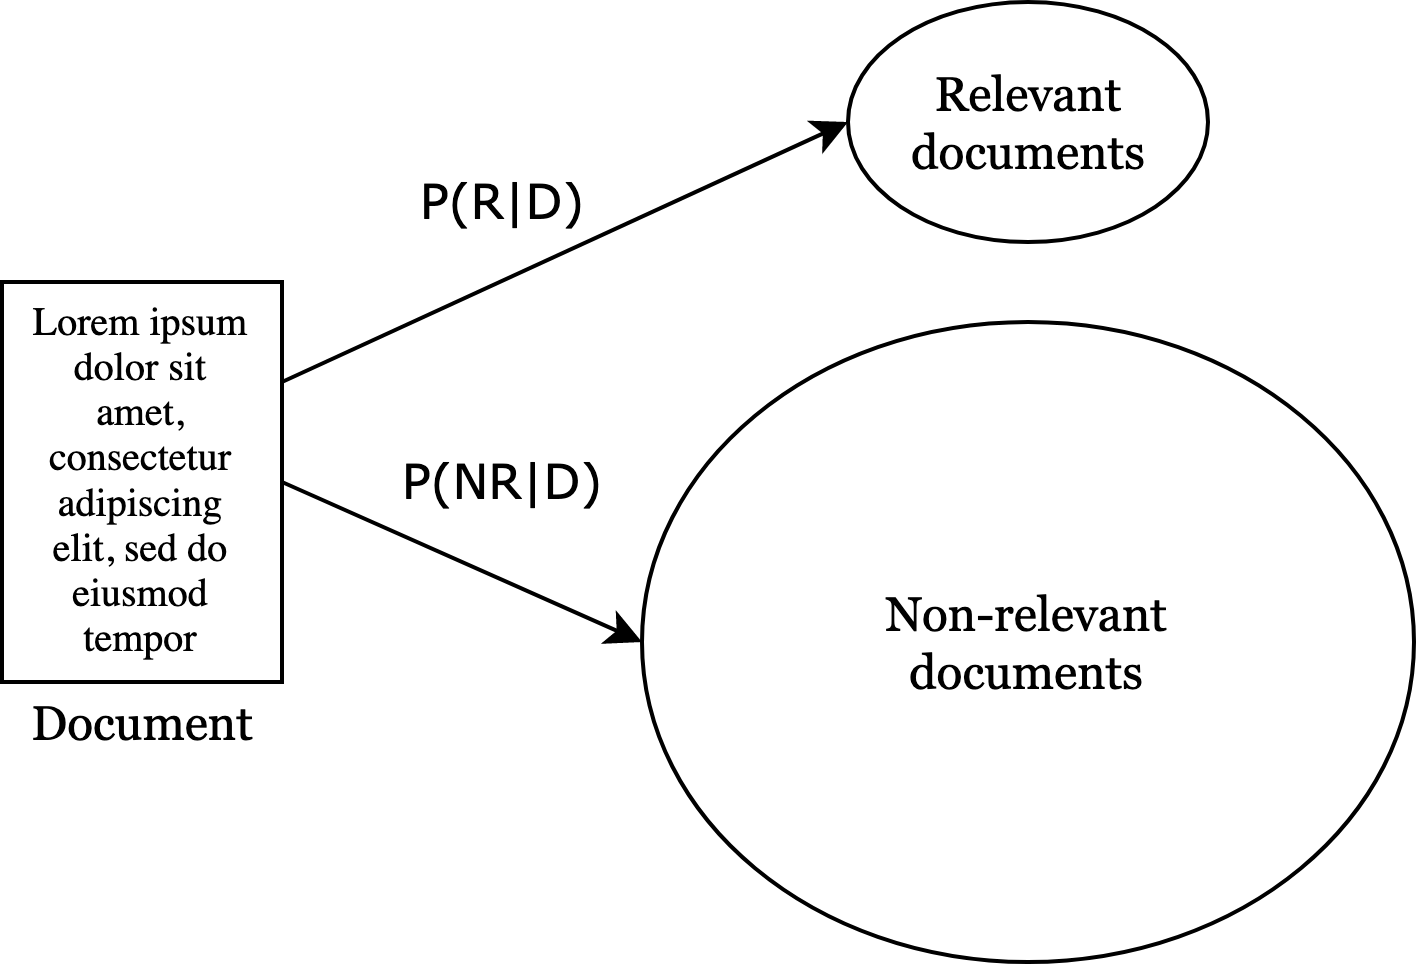
\includegraphics{images/probabilistic-ir.png}
\caption{Classifying a document as relevant or non-relevant\label{fig:probabilistic-ir}}
\end{figure}

\textbf{Probabilistic models} approach this problem from a probabilistic perspective. Using the well-known Bayes' theorem as their basis, they can lean on the robust foundation of probabilistic theory and apply many of its ideas to information retrieval. A general definition of the problem could be that there is a set of documents $D=\{d_1, ... d_n\}$ that should be categorized into two classes, relevant and non-relevant: $C=\{"R", "NR"\}$. To map the documents into those classes, a function $f$ is approximated $f: D \xrightarrow{} C$.

With Bayes' theorem this can modelled as a classification problem where the aim is to calculate the conditional probabilities of document being relevant $P(R|D)$ and non-relevant $P(NR|D)$, as shown in the Figure \ref{fig:probabilistic-ir}. It requires prior probabilities of any document being relevant $P(R)$ and non-relevant $P(NR)$, which could be measured by perhaps classifying some of the documents for a golden standard. The probability $P(D)$ is a normalizing constant that is the sum of all the probabilities of documents being relevant or non-relevant: $P(R)P(D|R) + P(NR)P(D|NR)$. To avoid calculating the conditional probability directly, we can turn this with Bayes' rule into Equation \ref{eq:bayes}.

\begin{equation}
\label{eq:bayes}
P(R|D)=\frac{P(R)P(D|R)}{P(D)}
\end{equation}
\vspace{-2pt}

A document would be classified as relevant when its conditional probability of relevancy would be higher than its non-relevancy: $P(R|D) > P(NR|D)$. This is referred to as the Bayes decision rule and the model Bayes classifier \cite{ir-in-practise}.

This model relies on the assumption that the documents can indeed be classified into relevant and non-relevant classes. While having a sound theoretical principle, in practise the relevancy of the documents is quite difficult to observe since it is subjective depending on the user. It will require advanced probabilistic models and a lot of data to accurately approximate users' perceptions of relevancy. Most large-scale search engines use probabilistic models and one of the most popular implementations is the Okapi BM25 model \cite{ir-in-practise}.

Codewebs avoids a part of this problem by using a user-specified seed set of documents that could be considered as the input for the search query. The system then retrieves the most relevant documents to that set with probabilistic modeling. This avoids having to write search queries but which might not be applicable to finding very specific patterns, only general approaches \cite{codewebs}. It is discussed in more detail in the Subsection~\ref{ssec:codewebs}.

An aspect we have omitted is the time and resources required to build the IR system. In most cases building your own search engine and probabilistic IR model might be too big of an undertaking unless it is the particular goal of the project. With CodeClusters, the building of a custom search engine for student code submissions was not considered as the particular aim of the project and instead already available libraries were used in the form of Apache Solr. 

\subsection{Vector space model}
\label{ssec:vsm}

As discussed in the previous subsection, one method to represent the documents is to use an algebraic model such as the vector space model. The simplicity of vector model has made it quite popular for all types of natural language applications beyond information retrieval to represent text documents. In vector space model, the documents and the search queries are represented as vectors in $s$-dimensional vector space, where $s$ is the number of unique terms. If the value of 1 was used when the document contained a specific term and 0 otherwise a binary term-frequency (TF) matrix would be produced, as shown in the Figure \ref{tbl:tf}.

\begin{table}[ht]
\begin{center}
\caption{Example binary TF matrix}
\label{tbl:tf}
\begin{tabular}{|c|c|c|c|}
\cline{1-4}
& \multicolumn{3}{ c|}{Documents} \\ \cline{2-4}
\hline
Term & $d_1$ & $d_2$ & $d_3$ \\
\hline % inserts single-line
\texttt{class} & 1 & 0 & 0 \\
\texttt{function} & 1 & 1 & 1 \\
\texttt{void} & 0 & 0 & 0 \\
$\vdots$ & $\vdots$ & $\vdots$ & $\vdots$ \\
\hline
\end{tabular}
\end{center}
\end{table}

Since this form is quite inflexible as it does not differentiate between how many times the term has appeared in a document, another possible weighting would be to use the raw term frequency count $tf_t=f_{t,d}$. Here $f_{t,d}$ is the frequency of the term $t$ in the document $d$. Other formats also exist. As discussed with the inverted index, this form is often non-optimal to use as such, which is why inverted indexes are used internally by the software.

The issue now becomes the ranking of the documents. A larger document that contains more terms will automatically rank higher than one that is smaller but which might be more relevant to the user. Therefore, a proportionate weighting is often added to this TF matrix in the form of inverse-document frequency.

\textbf{Inverse-document frequency (IDF)} is used to model the importance of the term relative to its occurrence in the documents. A term that can be found in all the documents will receive a IDF weight of 0, as it can not be used to distinguish between their differences. Its typical form is shown in the Equation \ref{eq:idf}.

\begin{equation}
\label{eq:idf}
idf_t=\log\frac{N}{n_t}
\end{equation}
\vspace{-6pt}

Where $N$ is the number of the documents, $n$ the number of documents the term $t$ appears in and $t$ the term in question. The TF matrix and IDF weights are often combined into one as the TF-IDF matrix, which is the TF weights multiplied by the IDF scores of the terms.

This format works relatively well for code as it does for text. One problem with the generation of a TF matrix is the pruning and normalization of the terms, which is amplified by natural language's ambiguity with synonyms and spelling errors. With code, the tokens are much less ambiguous although some tokens, like \texttt{while}-constructs, can be written in multiple ways.

A much bigger problem of the TF-IDF matrices is that the frequencies are unordered relative to how they occur in the documents, resulting in the loss of the original sequence. Hence this format is often called the "bag of words" model and it makes distinguishing structural patterns from the documents difficult. Another problem is every term having an equal importance in the weighting, whereas the teacher would probably rate a higher-level structure such as \texttt{class} or \texttt{function} as more important than variable assignments.

Having now enhanced the ranking of the documents, we must also find a way to score them in relation to the search query. This can be done with a similarity measure, of which the most popular one for vector space models is cosine similarity.

\textbf{Cosine similarity} calculates the cosine of the angle between two vectors which produces a value between 0 and 1, where 0 indicates orthogonality and 1 the exact same angle. This makes it very simple to use as it does not have to be otherwise normalized. Another benefit of cosine similarity is that since vectors of documents with a lot of terms become longer than the smaller documents', cosine similarity is not effected by their length. This proportionality mitigates one of the weaknesses of TF representation.

Scoring similarities for each document-query pair produces a similarity vector with which the documents could be ranked. On the other hand, if we scored similarities between each document pair we would create a similarity matrix as previously shown in the Equation \ref{eq:sim-matrix}, consisting of real numbers between 0-1 which is symmetric and has diagonal values of 1. This is the same format used in similarity detection as described in more detail in the Section \ref{sec:sim-detection}.

While we could save space by using an inverted index representation of the matrices, a problem often arises with terms that are popular but which do not offer a lot of predictive power. This becomes a problem even with a moderately sized dataset which makes computation inefficient. To reduce the dimensionality of the matrix we would want to remove those term vectors that do not improve our ranking.

\textbf{Singular value decomposition (SVD)} of $m \times n$ matrix \textbf{M} are the three matrices $\textbf{U}$, $\Sigma$ and $\textbf{V}^{T}$ as shown in the Equation \ref{eq:svd}. Here \textbf{U} and $\textbf{V}^{T}$ are two orthogonal matrices of size $m \times m$ and $n \times n$ and $\Sigma$ a diagonal matrix of size $m \times n$ with all the singular values of \textbf{M} as its diagonal values. In our case the $m$ would be the number of terms and $n$ the submissions \cite{intro-to-ir, mmds-2014-ullman}.

\vspace{-6pt}
\begin{equation}
\label{eq:svd}
\textbf{M}=\textbf{U}\Sigma\textbf{V}^{T}
\end{equation}
\vspace{-10pt}

When SVD is used for dimensionality reduction the aim is to decrease the size of the matrix \textbf{M} by removing the singular values that are very low relative to the others. This makes for a lot more efficient computation especially with large sparse matrices. In truncated SVD, which is what CodeClusters uses, an approximation of $\widetilde{\textbf{M}}=\textbf{U}_t\Sigma_t\textbf{V}^{T}_t$ is used where $t$ are the largest singular values of $\Sigma$. This is similar to Principal Component Analysis (PCA) where the least variance producing eigenvalues are discarded but in this case the data does not need to be centered thus it works well with the sparse TF-IDF matrices. Using SVD for TF matrices, such as TF-IDF, is often referred to as Latent Semantic Analysis (LSA) which is the finding of latent, underlying, relationships between the terms \cite{intro-to-ir, mmds-2014-ullman}.

In the Section~\ref{sec:sim-detection} similarity detection is discussed in more detail and in the Section~\ref{sec:clustering}, unsupervised learning methods to cluster the similarity or distance matrices.


\section{Analysis of program code}
\label{sec:analyzing-code}
A topic worth discussing is how teachers or programs can analyze code. Analyzing in this context can be a somewhat vague term as it can easily confused with assessment. In assessment student performance is evaluated by specific criterion and students provided feedback in either informal or formal manner. Most common categories of assessment are formative and summative assessment. In formative assessment teachers assess and provide feedback during the student's learning process in for example lab sessions as guidance how to approach to solve a problem. Summative assessment is conducted at the end of learning activity in attempt to summarize student's learning regarding a study objective, mostly in the form of grading. In our case, the provided feedback to the submissions could be considered as formative. The submissions themselves are the final work for a given exercise but the feedback is non-graded and aimed to improve the students' programming skills over the duration of the course \cite{assessment}.

Discussing \textit{analyzing} the student submissions however, we refer to the general approach of reviewing the submissions without having to grade them or to provide feedback. We are simply interested in finding patterns that could be generalized as insights. \textit{Reviewing}, in our context, can be considered as a form of analysis conducted to assess student work which can include feedback or grading but which in our case is done mainly to help teachers to understand the student programming patterns better. In research methodology the analysis methods are often categorized as either qualitative or quantitative. Qualitative research is the analysis of non-numerical data by finding general properties and patterns that can be described as written conclusions. Quantitative research on the other hand involves numerical data or data which has been quantified as such which is analyzed by statistical methods to draw conclusions about the researched subject~\cite{strengths-limits-qual-quant}.

Program code is non-numerical data that has been researched in various ways by either qualitative or quantitative methods. Analysis has been applied in educational context to researching facets such as students' debugging skills~\cite{static-analyses-in-py-courses}, learning~\cite{static-analyses-in-py-courses}, misconceptions~\cite{programming-errors}, predicted grades~\cite{analyzing-student-patterns} as well as code quality~\cite{static-analyses-in-py-courses, alamutka-2005-auto-ass-survey} and complexity~\cite{alamutka-2005-auto-ass-survey}. Most of them have been qualitative in nature but for at least complexity quantitative methods have also been applied.

\subsection{Manual review}
\label{ssec:manual-review}

As stated in the introduction chapter, manual reviewing of programming submissions is often unfeasible given their large volume. However, if manual reviewing is necessary to for example grade the submissions, the process is often standardized to maintain consistent evaluation criteria. Grading rubrics are guides that are used to list the criteria how to evaluate the submissions, the scale on which different aspects are scored, the common mistakes and their effect on grades as well as feedback phrases. Reviewing is often conducted by multiple people, and grading rubrics help to reduce the effect of subjective biases of the reviewers \cite{zimmaro-rubrics-2004, aalto-rubyric-2009}.

For us, manual reviewing can be a source of valuable insight to optimize the automatization of the process. A good and widely accepted grading rubric could help to develop the similarity measures to cluster the submissions or to detect outliers. Also, the grades and feedbacks of the manually reviewed submissions could be used for creating models to automatically grade and provide feedback to the submissions.

Creating models to automatically grade and provide feedback is, however, not trivial. In a study by Rogers et al.~\cite{rogers-auto-style-2014} four semesters worth of submissions of an introductory Python course are analyzed, totaling at 1500 submissions. All the submissions have been previously manually reviewed by teaching assistants (TAs), and given a score between 0 to 3 and varying amount of feedback. They list 26 features or criteria that they have extracted from the feedbacks which they consider important, and develop a supervised learning model to grade and provide feedback to submissions automatically. The accuracy of their results is very low, more akin to random classification, and they note that many of the features are not classified consistently \cite{rogers-auto-style-2014}.

As one of the causes for the poor accuracy they identify the inconsistency of the grades and feedbacks. The TA who graded and provided feedback to the submission was by far the biggest factor, making generalizations difficult. They argue that automating feedback with supervised learning is very difficult and with lack of precision, the tool they created would serve best for analyzing the submissions rather than automatically scoring them \cite{rogers-auto-style-2014}.

In a study by Glassman et al.~\cite{glass-feature-engineering} TAs were given 50 submissions and asked to cluster them manually in any manner they wanted to. They note that the TAs clustered the submissions by structural similarities, overlooking the presentational details of the code such as which library functions were used. Subsequently, the clusters between two TAs were found not to be very similar and an automatic clustering approach only started to match the manual clusters with high enough $k$, such as 15, using k-means clustering. While this would indicate that there are distinct structural patterns how submissions could be clustered, it also shows that generalizing a model that would work well for a wide range of teachers is hard \cite{glass-feature-engineering}.

In another study Luxton-Reilly et al.~\cite{luxton-sub-variation-2013} find by analyzing the submissions of 10 simple program code exercises of an introductory CS course, that the variation between the submissions could be categorized into three distinct and hierarchical types. Structural variation is the highest level with the most variation, which is the control-flow structure of the program, represented by a control-flow graph. Syntax-level is the second highest, which is the variation of used program syntax that does not contribute to control-flow and it is only considered if the two submissions share the same control-flow structure. At the lowest level, if the syntax of the submissions would also match, the presentational-level would be the variation in aspects such as difference in formatting, the exact used tokens and their order \cite{luxton-sub-variation-2013}.

This study could indicate that in order to cluster the submissions by their similarities, the methods should have to be specified to certain variation level Also, the feedback could be defined as either belonging to a certain variation level or as a synthesis of multiple levels. Using a similar ontology might help writing better feedback and creating more accurate similarity detection models.

To summarize, manually reviewing the submissions is a good first step when building automatic grading or feedback system. The grades and feedbacks might be correlated to some structural patterns in the code yet their use for modeling can be problematic. The subjectivity of the reviews and their possible low quantity would not perhaps lend itself for good classification models. Analyzing and understanding the qualitative criteria how people intuitively cluster the submissions by hand would still seem very valuable. 

\subsection{Programmatic review}

Automatic analysis tools are important applications for both code and natural language text to evaluate their quality. In the context of program language code these are commonly categorized as static or dynamic analyzers, where static analysis is the analysis of the programs without executing them and dynamic analysis during their execution \cite{static-dynamic-hybrid-analysis}. Dynamic analysis is mostly concerned with performance although OverCode uses dynamic analysis of the execution graphs to canonicalize variable names\cite{overcode}. The automated tests could be considered as a form of dynamic analysis. Due to the difficulty of applying dynamic analysis as it is heavily dependent on the programming language and its execution model, we shall focus on only the static analysis and its applications.

One popular type of static analysis tool is a program called "linter", the name derived from a Unix C style checker named \texttt{lint}~\cite{lint-1988}. It provides small feedback messages how to properly format or fix segments of the code that it could even do automatically. This helps developers to maintain uniform style, reduce maintenance, enhance readability and to avoid errors in their code \cite{lint-1988}. More advanced static analyzers can find very concealed and complex problems with the codebase based on extensive data and heuristics on what causes bugs~\cite{fb-static-dynamic-analysis}.

Could the teachers' reviewing of the submissions be defined as static analysis of poor formatting, inefficient computation or bugs in the code? Unlike with the industrial grade static analyzers, the motivation for teachers is pedagogical and not the heavy constraints of having to ship robust and efficient code in a standard manner. It could even be seen as counterproductive to require the same standard of quality from the students as from highly skilled software engineers. And even if the students were able to fix their code with the help of a very good static analyzer, how much would they benefit from the mechanical task of blindly following the tips of the analyzer?

Certainly, some standard of quality has to be required from the students yet the justifications for it are necessary. Adding a strict style checker as part of the automated test suites would probably not be immensely helpful for helping the students to learn, who would be overburdened by having to solve the exercises and fix seemingly arbitrary style errors as well. Creating a static analyzer with pedagogically good error messages could be challenging, but they have been implemented in some cases \cite{static-analyses-in-py-courses, fox-roy-autostyle-msc-2016}. We outline the benefits of static analyzers as a possible future research topic in the Subsection~7.1.2.

A major obstacle in automating this form of qualitative analysis would be its subjectivity. For example, generalizing an aspect such as complexity as overly long and verbose code is problematic as it could happen that longer code was more readable than shorter. Therefore, it seems implausible that teachers could be able to create a set of feedback messages and patterns that would be comprehensive and specific enough and also apply to all the exercises in a given course. Specifying the analysis on exercise basis would probably provide teachers more flexibility and freedom in generating the messages and their patterns.

In the context of a single exercise, this method might work relatively well. However, this would require considerable time and effort from the teachers to find patterns from the code that were consistent enough so that they could be used as indicators of for example misconceptions or problems in the code. Creating and maintaining a very large collection of these patterns and their messages would seem very similar to creating an additional set of automated tests, which benefits and drawbacks were discussed in the introduction chapter. Another question is, would the students appreciate such automatization? In theory, better feedback should be beneficial to students' learning and motivation but if the students would see the messages only after they had received their points, they could see it as extra-work. Therefore, the exact approach to implement static analysis would have to be carefully planned.

Crow et al. note that in many introduction programming courses code quality is not even necessarily taught to the students \cite{crow-code-quality-2020}. Therefore, the students might not even know how to write readable code that is clean, modular and uncomplex. A static analyzer could indeed help to inform students about the quality of their code, but it also should be the responsibility of the teachers and the course material.

Instead of a static analyzer, an intelligent tutoring system (ITS) could provide more general real-time formative feedback to the students while they were solving the exercises. Rather than only parsing patterns and providing canned messages, it could be incorporated as a more holistic help that used the metadata of failed submissions and historical student performance. Thus it could provide tailored help whenever student failed to progress in the exercise or just general advice, similar to how students would receive help in lab sessions. Creating an ITS would require extensive data of incomplete or buggy submissions at points where the students have struggled the most. Also it would require substantial effort and expertise to build, and it might not scale well for exercises with large solution spaces \cite{glassman-reusable-feedback, its-2020}.

Glassman et al. for example propose MistakeBrowser and FixPropagator that enable the analysis of failed submissions to find the shortest number of transformations that would fix them, and allow teachers to provide feedback to students for that specific problem \cite{glassman-reusable-feedback}. Ngueyn et al. also propose a system for real-time feedback that is built on top of Codewebs \cite{nguyen-real-time-feedback}. The benefit of ITS compared to static analyzer would be the depth of the possible feedback provided to the student, yet they are not mutually exclusive. What, however, would be important, is the real-timeness of the feedback. If the feedback was delayed until the student had submitted their code, or by days or weeks, the student might not internalize it very deeply. Real-timeness might also be more effective in preventing the students from forming bad habits.

\iffalse
xcite luxton Understanding Semantic Style by Analysing Student Code Who also found 16 different semantical indicators of potential lack of knowledge.

Data-driven Feedback
Treating feedback generation as a classification task allows us to address RQ1 and evaluate the extent to which SourceCheck agrees with (predicts) the feedback of human tutors. The results of this evaluation would be difficult to interpret without a baseline for comparison

RQ1: How well does SourceCheck’s feedback agree with ideal human tutor feedback? SourceCheck agrees with approximately half of ideal tutor feedback provided in Phase I, almost as much as another human tutor, with SourceCheck achieving a recall 76 and 88\% as high as TC on GG and SQ respectively. This does not necessarily mean that SourceCheck’s feedback is almost as good as a tutor’s. It is possible that when SourceCheck’s feedback diverges from a tutor’s, it does so in a less useful way than when another tutor does so; however, this is difficult to investigate without some direct measure of hint quality (e.g. [8]). For now, we can say that these results suggest good potential for data-driven feedback generation, in that ideal tutor feedback is frequentlycontained in the set of edits generated by SourceCheck.
\fi


\section{Representations of program code}
\label{sec:representations}
We already discussed how to represent unstructured data such as code in an IR system in the Section \ref{sec:ir}. In vector space model, each document was transformed into an array of tokens that were represented as vectors of frequencies. Yet because program code is in fact instructions for the compiler how to run the program, it has hierarchical structure that is very precisely defined by its grammar. When the compiler parses the code, it transforms it into one or multiple intermediate representations, such as abstract syntax tree (AST), that help in type checking, optimizing and analyzing the code. Higher-level intermediate representations are easier to optimize and manage than lower-level representations, which is why syntax trees are often used instead of linear representations or machine code \cite{aho2007compilers}.

Another form to represent code is the control-flow graph that represents the execution path of the program. They are used by the compiler to analyze and optimize the program, as well as how to schedule and allocate memory \cite{engineering-compiler}.

And as described in the IR Section, the code could also be treated as an array of string tokens. It can be generated by parsing the AST and then processing it in depth-first fashion by pushing its nodes into an array. While it loses its original tree-structure, arrays provide much greater flexibility in using various machine learning models. Using n-grams instead of single tokens allow retaining some of the original structure.

This section goes through these three selected representations in more detail to understand their differences, and what benefits and drawbacks each have for representing code. Most of this section is based on the books \textit{Engineering a Compiler: 2nd Edition} (2013) by Cooper et al.~\cite{engineering-compiler} and \textit{Compilers: Principles, Techniques, and Tools: 2nd Edition} (2006) by Aho et al.~\cite{aho2007compilers}.

\subsection{Abstract syntax tree}
\label{ssec:ast}

Executing program code is a multi-staged process that is done differently in many programming languages and environments. Some languages, like Java, use just-in-time (JIT) compilation and run the program on a virtual machine. Others, such as C, are compiled to a single executable binary that is customized for a specific operating system and processor architecture. But regardless of the details of the process, in-between the parsing and executing the program, one or more intermediary representations (IR) for code are used \cite{aho2007compilers}.

In general, the program code is first parsed into a stream of tokens, the basic syntactical units of the language, by a lexer. Then, the tokens are parsed into a parse tree by a parser following the grammar of the programming language. Because parse trees contain the whole derivation of the grammar, they can become very large and bulky which is which they are often transformed into more compact abstract syntax trees (ASTs) \cite{aho2007compilers, engineering-compiler}.

ASTs eliminate much of the redundancy of the parse trees and offer a good abstraction level for the compiler to analyze and optimize the program. Some compiler architectures use ASTs for executing the program while others transform it to another, lower-level IR, before execution. The AST could be turned into a directed acyclic graph (DAG) which is sometimes done by the compiler, but for us a normal undirected graph would be the most flexible to use. As AST is a tree all its directed edges are from the parent nodes to their children which makes that information redundant. Therefore, using an undirected graph would be preferable as it is more efficient to use and available to more graph algorithms \cite{aho2007compilers, engineering-compiler}.

While a graph of AST might be easier to use than tree, from modeling perspective the size of the graph would still be too large. Many of the graph algorithms, such as tree-edit distance, are not exactly fast with worst case complexity of $O(n^4)$ \cite{ted-tutorial-2018} which might lead to very slow run times. A lot of the tokens might also not contribute any meaningful signal in the detection of outliers or similarities, and thus they could be regarded as noise. Semantically similar tokens are also prevalent in ASTs, which makes discerning similarities hard. 

As a solution to this problem systems such as MistakeBrowser~\cite{glassman-reusable-feedback} and Codewebs~\cite{codewebs} standardize the ASTs by removing the less important tokens, which could be seen corollary to removing stop-words in natural language processing (NLP). Then, similar tokens are transformed into a single representation, such as all \texttt{for} and \texttt{while} tokens becoming \texttt{loop} tokens.

JPlag, a Java plagiarism detection library, has a list of 39 tokens that it only considers in their detection algorithm and a larger set of 82 tokens that can be optionally selected by the user. They note that while the larger set does capture more structural features, it also increases noise which might lead to misclassifications \cite{jplag}. CodeClusters allows the use of three sets of tokens: language keywords, all available AST tokens and a version of JPlag \cite{wahlroos-2019}. The JPlag version seemed to produce the most reliable results.

To summarize, ASTs offer the full syntactical structure of the program in a hierarchical form. Because they can be rather large and noisy from the modeling perspective, they are often pruned and standardized before used in models. This helps to combat the curse of dimensionality and to increase accuracy in detecting semantically similar code. Since the results between the different sets of used tokens might vary, they have to be carefully crafted and analyzed by for example offering multiple different sets for the user to choose. 

\subsection{Control-flow graph}

Knowing the execution paths of a program is very helpful when analyzing it for optimization. Normally, this is modeled as a control-flow graph (CFG), which is a directed cyclic graph of all the possible execution paths a program may take during its execution. Its nodes are the basic blocks of a program that are sections of code always run in sequence with control entering at its first operation and leaving at the last. Every edge in the graph is a possible transfer of control between the blocks \cite{control-flow-analysis, aho2007compilers, engineering-compiler}.

CFGs have traditionally been used for compiler optimization and static analysis, as they portray the actual execution of the program, unperturbed by the syntactical noise \cite{control-flow-analysis, engineering-compiler}. Cyclomatic complexity uses CFGs in its calculation of complexity \cite{mccabe-1976}.

In our case, CFGs might be better suited for structural analysis of the submissions compared to ASTs. They remove many of the noisy details of formatting and syntax leaving out the actual behavior of the program. CFGs have also been used to label variations between student submissions \cite{glass-feature-engineering, luxton-sub-variation-2013}.

Losing the tokens, however, also implies losing the ability to detect any syntactical similarities. This would decrease the overall applicability of models that use only CFGs. Attempts have been made to join the two into a graph that shows the control flow structure of the program while retaining many of the tokens of the AST. Control-Flow Abstract Syntax Tree (CFAST) \cite{cfast} for example models the control structure of the code by pruning ASTs to only contain the tokens that contribute to the control flow of the program.

\subsection{Token array}
\label{ssec:array}

As described in the vector space model Subsection \ref{ssec:vsm}, code can be transformed into a sequence of tokens $d=(t_1, ..., t_n), t\in L$ where $L$ is the set of available tokens. Being an ordered list, it could be stored as an array and trivially transformed into a term-frequency matrix. From the compiler perspective, array is not very sufficient for representing code as it loses the hierarchical structure of the program. Only at the beginning of the compilation step the tokens are parsed to an array by the lexer. Therefore, compilers do not output it as such, and it has to be generated outside of the compiler by processing the AST using depth-first search and pushing its nodes into an array \cite{engineering-compiler, aho2007compilers}.

While lacking the structure of the graph, the array offers many exciting opportunities from modeling perspective as it is very similar to text, hence allowing the use of many text mining or NLP algorithms. Its linearity also makes it fast to process compared to graphs, which are not as easy to process in parallel\cite{parallel-graphs-2018}.

However, because the original ASTs were hierarchical trees, one-dimensional arrays lose a lot of structural information about the program. This might lead to poor performance in detecting structural similarities. Especially with representations such as the TF-IDF matrix, where the vectors are treated unordered thus losing not only the hierarchical structure but also the sequential order.

Some systems, such as JPlag, try to alleviate this problem by using separate tokens for the start and end of statements, such as "BEGIN\_IF" and "END\_IF" \cite{jplag}. This helps detecting nestedness in the data and in combination with n-grams, which is described in the Subsection \ref{ssec:ngrams}, the tokens are able to retain some of the original structure and order.


\section{Software metrics}
\label{sec:metrics}
As mentioned in the Section~\ref{sec:analyzing-code}, code can be quantified into numeric values which are in the context of programming languages called metrics. While their purpose is good and from modeling perspective numerical values are much easier to process than text, their indicative power cannot often be verified. Therefore, a consensus exists that metrics should be treated with a healthy amount of scepticism, and be treated as guidelines rather than absolute thresholds.

\subsection{Halstead complexity measures}

The earliest published metrics are the Halstead complexity measures by Halstead (1972, 1977), \cite{halstead-1972, halstead-1977} that are based on the assumption that code can be measured, analogous to the measurement of physical properties of gases and matter. The earliest known plagiarism detection system of code by Ottenstein~\cite{ottenstein, jplag} (1976) was based on Halstead measures.

What Halstead proposed was formulae to calculate properties such as vocabulary, volume, effort but also time to code and the number of derived bugs, all derived from counting operands and operators of the program \cite{halstead-1977}.

\begin{center}
$\eta_{1}=$ the number of distinct operators

$\eta_{1} =$ the number of distinct operands

$N_{1} =$ the number of total operators

$N_{2} =$ the number of total operands
\end{center}

The vocabulary of the program would be for example $n=\eta_{1} + \eta_{2}$ and program length $N=N_{1} + N_{2}$ \cite{halstead-1977}.

While at the time of their publication the quantification of code was a novel idea, the later research has shown that the predictive power of the measures is questionable \cite{halstead-in-oop-2004, halstead-emperors-clothes-1982}. In fact, it is debatable do any of the measures hold up to scrutiny with modern programming languages and very large repositories of source code \cite{halstead-in-oop-2004}.

Interestingly, a neural network clone detection system Oreo by Saini et al. uses 24 metrics as its features which include 3 of Halstead's measures and which appeared to have worked well in detecting challenging clones~\cite{oreo, chaiyong-2018}. Perhaps neural nets could benefit from the very small signal of the measures as part of their massive datasets, but the research on the matter has not been conclusive.

With CodeClusters, however, the Halstead measures were omitted due to their poor predictive power and the possible confusion arising from the naming of the measures.

\subsection{Cyclomatic complexity measure}

Around the same time as Halstead proposed his measures, cyclomatic complexity measure was published by McGabe (1976)~\cite{mccabe-1976}. Instead of counting the operators and operands, cyclomatic complexity counts the nodes, edges and components of the control-flow graph of the program as an indicator of its complexity. Its function $V$ is defined in the Equation \ref{eq:cc}.

\vspace{-10pt}
\begin{equation}
\label{eq:cc}
    V(G)=N-E+2\cdot P
\end{equation}
\vspace{-10pt}

Where $N$ is the number of nodes, $E$ the number of edges and $P$ the number components in the directed graph $G$.

The arguments for its use were based on the observation that in order for unit tests to gain full test coverage of the program, all the combinations of its execution paths should be tested. Therefore, cyclomatic complexity would directly correlate with the minimum number of tests the program would require \cite{mccabe-1976}.

Since its publication, the cyclomatic complexity has endured in software engineering research better than the Halstead measures, yet its popularity has decreased noticeably \cite{halstead-in-oop-2004}. Main criticism against it is that it is a poor predictor of complexity per se. One can even say that to call it complexity when its purpose is to measure the minimum number of required tests misleading, as long code with higher cyclomatic complexity might actually be less complex than code that is short but obtuse \cite{shepperd-cc-1988}.

One research even concludes that with a large enough program, the lines of code reach almost perfect linear relationship with cyclomatic complexity~\cite{cc-is-loc}. Hence, cyclomatic complexity loses any explanatory power as the correlation between the two becomes close to 1. For the 10\% of code that deviates from this a closer inspection might be in place, but in general it argues that lines of code is as good of a measure of complexity as is cyclomatic complexity. This has been noted in other studies as well \cite{shepperd-cc-1988}.

Due to its prevalence in static software analyzers and therefore being easy to implement, CodeClusters allows the use of cyclomatic complexity as a parameter in its search interface. While it can produce ambiguous results, the teachers might also find outliers that contain unique solutions.

\iffalse
CodeClusters also includes NPath metric which was created as an improvement to cyclomatic complexity.
\fi

\subsection{Lines of code}

One of the simplest metrics to calculate for any program is the lines of code (LOC). The exact way it is calculated has not been standardized, although most commonly only the non-blank and non-comment lines are counted. It is heavily effected by the programming style and a verbose style that uses many lines will accumulate magnitudes higher LOC than style which is terser. Also, it is not able to discern structural differences between two programs that both share the same LOC~\cite{abc-metric}.

Because of its simplicity to implement, CodeClusters includes LOC as part of its search parameters. It might serve a purpose in outlier detection given that most submissions will probably be close to the average LOC.

\subsection{Assignments, branches, conditionals metric}

Assignments, Branches, Conditionals (ABC) metric was created as an improvement to LOC that would, instead of counting lines, count the important structural parts of the program. It is a vector $\mathbf{v}=\begin{bmatrix} A & B & C \end{bmatrix}$ where each value is counted by methods specific to a given programming language. The resulting 3-length vector can then be used as such or by its magnitude $|\mathbf{v}|=\sqrt{A^2+B^2+C^2}$. It was designed to overcome the major weaknesses of LOC by being able to discern structural differences and not being heavily effected by the coding style. It is, however, dependent on the methodology how it is counted and each programming language and implementation might follow a different methodology \cite{abc-metric}. It has been used in some automatic student feedback systems \cite{fox-roy-autostyle-msc-2016}.

Although interesting, ABC metric was ultimately not implemented in CodeClusters as it already had a good number of metrics. Also the time required to implement it at the expense of other, more critical features, was a concern.


\section{Similarity detection}
\label{sec:sim-detection}
Similarity is an abstract concept that is hard to describe in exact terms. Philosophically, similarity of objects is only a matter of framing - all submissions are code and therefore similar. Yet for us a more precise definition would be more usable.

We shall define similarity as the similarity of the documents' elements and structure when they are represented as trees, graphs or arrays. We normalize this similarity value $s$ as $\{ s \in \mathbb{R} \mid 0\leq s \leq 1\}$ where 1 indicates equality and 0 total dissimilarity. The range $[0,1]$ is arbitrary but chosen for its good mathematical properties. In this context similarity distance would mean the opposite of similarity, which can be defined as $d = 1 - s$. Similarity detection would be the applying of a similarity scoring function, such as $sim : (a, b) \rightarrow [0,1]$, for a set of documents $D=\{d_1, d_2, ..., d_n\}$ to create a similarity matrix with the scores computed for every document in relation to every other document, as shown in the IR Section Equation \ref{eq:sim-matrix}.

Most of the research in similarity detection of program code has focused on the detection of plagiarism, software license violations and clones. To differentiate between the similarity types, three levels have been proposed: purpose, algorithm and implementation level \cite{zhang-towards-plag-det}.

If two programs both sort numbers by ascending order, they can be considered similar at the purpose level. If they share the same algorithm, at algorithm level, and if their implementation of the algorithm is the same, at implementation level. Due to the difficulty of deciding whether two programs are equal at the purpose or algorithm level, most similarity methods work only at the implementation level \cite{chaiyong-2018}. If we expect every student to have solved the same exercise, we could already assume them to be same at the purpose level.

Similarity detection has been a popular approach for providing clustered feedback to students \cite{overcode, codewebs, divide-and-correct, fox-clust-leverage-2015, fox-roy-autostyle-msc-2016, stanford-million, survey-feedback-gen}. An explanation could be that it closely simulates the natural process how humans would group the submissions together if they were to provide shared feedback to many submissions at once. An alternative could be to use classifiers to provide feedback or rule-based analyzers. Deciding how the similarities are calculated is crucial in producing accurate results, yet as discussed in the Section~\ref{sec:analyzing-code}, there might be multiple similarity levels and their measurement would be susceptible to subjective biases by human reviewers.

Systems such as OverCode, Codewebs and Divide and Correct all use similarity detection and their results are used to cluster the submissions. Many of the systems use derivations of ASTs as their representation, but the used similarity measures vary a lot. OverCode uses a custom algorithm that matches the canonicalized stacks together, Codewebs uses probabilistic semantical equivalence to find the most used context for given AST subtree and Divide and Correct uses multiple feature vectors which are compared using cosine similarity \cite{overcode,codewebs,divide-and-correct}.

The trade-offs of each method are their accuracy and generalizability outside that specific dataset, yet it is hard to say what method would be the most balanced given the wide range of possible data and representations. The most flexible approach could be to offer multiple methods that can detect similarity at different levels, which we discussed previously in the Section \ref{sec:analyzing-code}.

Another use case for similarity detection is plagiarism detection, which is not discussed in the context of this thesis. With good similarity detection mechanism finding very similar student submissions should be trivial but applying it to publicly available code on internet would be challenging \cite{simon-better-ngrams-2020}.

Next, we present a few of the most popular and interesting similarity detection methods for code, namely tree edit-distance, greedy string tiling and n-grams. A major area that is omitted is neural network based systems, such as Oreo~\cite{oreo}, since while promising they require very in-depth technical analysis which is not possible in the scope of this thesis.

\subsection{Tree edit-distance}
\label{ssec:ted}

Its best-known version proposed by Zhang et al. (1989) \cite{zhang-et-al-1989} tree edit-distance (TED) is the minimum number of edit operations required to transform a tree into another tree. The operations to edit the tree in the original paper were threefold: \texttt{insert}, \texttt{delete} and \texttt{rename}. Some versions might use more operations.

Since TED only computes the distance between two trees, for similarity detection the algorithm has to be computed for all the unique pairs of documents. These are for a set of documents $D$ all the combinations of two $\binom{D}{2}$. This results in a symmetric edit-distance matrix with diagonal values of 0, the edit-distances being positive integers $e \in \mathbb Z_{\ge 0}$. They could be normalized into similarity distances between $[0, 1]$ by dividing them by the largest edit-distance, but since the relationship would stay linear this only matters if the clustering algorithm requires it.

The algorithm itself is quite long and complicated and it would need substantial explanations on its behavior, so we shall omit a detailed analysis and summarize it as a recursive function with two inner loops that store the calculated distances in a large edit-distance matrix, and backtracks the shortest path once the matrix has been completed. But unless optimizations are in place the algorithm will iterate over every possible combination the tree $a$ could be transformed into tree $b$ \cite{zhang-et-al-1989, ted-tutorial-2018}.

Zhang et al. note that the worst-case time complexity of the algorithm is $O(m^2\cdot n^2)$ where $m$ and $n$ are the number of nodes in the trees, which with two equally sized trees would become $O(n^4)$. Using optimizations, such as hash tables and dynamic programming, the space complexity of the algorithm becomes however $O(mn)$ \cite{zhang-et-al-1989, ted-tutorial-2018}. Later advancements have brought the time complexity to $O(n^2m(1+\log \frac{m}{n}))$ \cite{ted-demaine}.

This makes applying it quite problematic as it does not scale very well to larger datasets. Many plagiarism detection and educational clustering systems use TED as their similarity detection algorithm, yet many note its poor scalability to be one of the main issues with the method
\cite{stanford-million, fox-clust-leverage-2015, fox-roy-autostyle-msc-2016}. 

Its benefits lie in its hierarchical behavior; for example, removing a higher-level node with many children will take multiple operations, as every child has to be removed or moved first. This automatically weights the algorithm so that structures higher in the tree have larger impact on the similarity calculation. Also, while the worst-case complexity in theory is quartic, Nguyen et al. note that in practise for their student submissions it is only quadratic \cite{stanford-million}.

To improve the detection of structural differences, it might still be better to add a separate cost function that would define different costs for different operations and nodes. For example, removing lower-level node such as variable assignment should probably have a lower weight than removing a structure such as \texttt{class} or \texttt{function}. Fox et al. propose this weighted TED for their similarity detection of programming submissions and note that it performs better than the non-weighted version \cite{fox-clust-leverage-2015}.

For CodeClusters we tested TED with our moderately sized 110 submission test dataset, yet the algorithm performed very slowly taking approximately 10 minutes each execution. With better, lower-level and parallelized implementation it could perhaps be a lot faster to run but due to the limited available resources to fix it, it was not included.

\subsection{Greedy string tiling}
\label{ssec:gst}

Another popular method for plagiarism detection is greedy string tiling (GST) algorithm, originally proposed by Wise (1993) \cite{wise-gst-1993}. As indicated by its name it is commonly used with strings, but since a string is only an array of characters it can be modified to work with token arrays. Two of its most popular implementations are the JPlag and YAP3 plagiarism detection libraries \cite{jplag, yap3}

The issues with GST are similar to TED which are its high worst-case complexity and inability to differentiate with token types or their operations. GST has a worst-case complexity of $O(n^3)$ but using an optimization in the form of Karp-Rabin algorithm to store the subparts of input strings, or arrays, as hash values in a hashtable, the practical worse case becomes between $O(n)$ and $O(n^2)$ \cite{wise-gst-1993}. Yet unlike TED, GST does not allow weighting of the tokens which makes it less flexible for structural similarity detection.

For CodeClusters, we evaluated GST but the time it would have required to properly implement it was deemed too long. Also, the problems with TED indicated that the high worst-case complexity might be a big problem. By analyzing the clusters from the TED and n-grams models, we found that the algorithms detected mainly presentational similarities and not very deep structural patterns. This could mean GST is especially poor fit due its limited capability in detecting higher-level structure.

\subsection{N-grams}
\label{ssec:ngrams}

N-grams is not exactly a similarity detection method in itself, but a method to represent strings or arrays in a form that captures some of their sequential structure. A formal definition would be that n-grams of a string are all the $n$ length contiguous substrings. For example, n-grams of string "aabc" would be $\texttt{2-grams}(\text{"aabc"})=\{\text{"aa"}, \text{"ab"}, \text{"bc"}\}$ with $n=2$ \cite{ir-in-practise, chaiyong-2018}.

N-grams is widely popular in natural language plagiarism detection and as a method to represent text in general, and they are often used with vector space representation which was described in the Subsection \ref{ssec:vsm}. The similarity between two vectors could be measured with various methods, but the most popular similarity measure is cosine similarity \cite{ir-in-practise, chaiyong-2018}.

The main strengths of n-grams are its flexibility and efficiency. Compared to TED and GST, generating n-grams for a document is a $O(n)$ operation that is computed only once per document, not every document pair. After n-grams have been generated they can be transformed into a TF-IDF matrix which can be processed with vectorized operations.

The weaknesses of array representation were mentioned in the Subsection \ref{ssec:array}, which come down to its lack of hierarchical structure that makes discerning higher-level patterns difficult. What n-grams is capable of, however, is discerning local sequential structure of the tokens which can be combined with the results of multiple different sized n-grams. Using specific tokens to indicate start and end of statements work to some extent as demonstrated by JPlag, yet they are lacking in power.

A novel improvement for AST-based n-grams is proposed by Karnalim and Simon which instead of creating n-grams sequentially from the array, it generates them following the hierarchical structure of the tree. For example, a sequence of tokens such as \texttt{PARENT}, \texttt{CHILD\_1}, \texttt{GRANDCHILD}, \texttt{CHILD\_2} would under sequential processing of 2-grams become: \texttt{(PARENT, CHILD\_1)}, \texttt{(CHILD\_1, GRANDCHILD)} and \texttt{(GRANDCHILD, CHILD\_2)}. Whereas hierarchical processing would generate: \texttt{(PARENT, CHILD\_1)}, \texttt{(PARENT, CHILD\_2)} and \texttt{(CHILD\_1, GRANDCHILD)} \cite{simon-better-ngrams-2020}.

CodeClusters uses n-grams as its main similarity detection method which works moderately well, although the clusters it produces are perhaps even too similar leaving out a large portion of the dataset unclustered. Therefore, the granularity of the used ASTs should probably be lowered to better capture structural aspects instead of presentational variations. Using hierarchical n-grams might also result in improvements.


\section{Clustering}
\label{sec:clustering}
The previous section presented a few of the possible methods to produce similarity or distance matrices of the submissions. While the matrix could be analyzed as such to find the lowest or highest values to cluster the submissions, this method is not very scalable or flexible and it would require manual input from the teachers.

The values of the matrix could be defined as a set of vectors $X=\{\mathbf{x}_1, ..., \mathbf{x}_n\}, \mathbf{x}_i \in \mathbb{R}^s$ in $s$-dimensional space where $s$ is the number of submissions. Subsection \ref{ssec:ir-system} discussed probabilistic IR models that were a form of supervised learning to classify the submissions into either relevant or non-relevant classes: $C=\{"R", "NR"\}$. Yet for the similarity data we have not defined any classes to classify them with. Subsection \ref{ssec:manual-review} analyzed how plausible manually classifying the submissions would be, but the research showed this approach not to be very reliable. Therefore, we are limited to unsupervised learning methods, a category of machine learning, where unlabeled data, such as code submissions, is discerned for patterns or clusters \cite{data-mining-2011}.

Clustering is a subcategory of unsupervised learning in which the datapoints are automatically separated into as similar clusters as possible, maximizing the dissimilarity between the clusters. The clustering algorithms can be categorized in multiple ways but we divide them into three major types: hierarchical, partitioning and density-based. They each follow a particular approach how they form the clusters and how they expect the datapoints to be distributed \cite{optics-1999, data-mining-2011}.

With hierarchical clustering each point is processed individually by their proximity to other points or clusters and continued until all points have been separated or joined into one cluster. This results in a hierarchical tree from which the most optimal splits of the points can be found and the clusters that seem the most prominent. Partitioning algorithms try to divide the points into regions belonging to a certain cluster. Density-based algorithms use the density of the points to create clusters that are separated by lower-density boundary regions \cite{data-mining-2011, jain-50y-kmeans-2010, optics-1999}.

The benefits of each approach depend on the used data and on how one would like the data to be clustered. In the extent of this thesis, we shall be discussing in more detail only k-means, DBSCAN and OPTICS clustering algorithms. They were selected for their popularity and use in other student submission clustering studies \cite{divide-and-correct, fox-clust-leverage-2015, glass-feature-engineering, fox-roy-autostyle-msc-2016}. We also evaluated them with CodeClusters using n-grams based similarity detection model and the experiments found none of them to be distinctively better than the others. The model and clusterings were ran with various parameters and the clusters were analyzed manually and by their silhouette scores. Silhouette score measures the degree how distinct the clusters are based on the distances of the points in and outside the clusters. A low score would indicate little difference between the clusters and higher score more distinct and separable clusters \cite{fox-clust-leverage-2015}.

For the teachers the choice of the algorithm might not be of much importance since they are only interested in the analysis of the clusters and the submissions. But during the experimentation with CodeClusters it became evident that clustering cannot be completely abstracted from the teachers, as the differences between different algorithms can be substantial. Also, some of the teachers might enjoy changing the clustering parameters manually by themselves. We included 4 clustering algorithms in CodeClusters which were k-means, DBCSAN, HDBSCAN and OPTICS.

\subsection{K-means}
\label{ssec:kmeans}

Its idea going back to 1950s, k-means is a partitioning clustering algorithm that uses cluster center points, centroids, to assign data points into clusters. Its parameters are a set of observations $X=\{\mathbf{x}_1, ..., \mathbf{x}_n\}, \mathbf{x}_i \in \mathbb{R}^d$ of vectors in a $d$-dimensional space and the used number of clusters $k$. A distance metric can be given optionally as third parameter but squared Euclidean distance is commonly used: $d(\mathbf{x}, \mathbf{y})=\sum^{n}_{i=1} (\mathbf{x}_i - \mathbf{y}_i)^2 + ... + (\mathbf{x}_n - \mathbf{y}_n)^2$ \cite{islr-2014, jain-50y-kmeans-2010}.

\begin{algorithm}
\caption{K-means algorithm \cite{ir-in-practise}}\label{alg:kmeans}
\begin{algorithmic}[1]
\Require Set of datapoints $X=\{\mathbf{x}_1, ..., \mathbf{x}_n\}$
\Require Number of clusters $k$
\Procedure{K-means}{$X,k$}
  \State $L[1], ..., L[n] \gets \Call{SampleRandomCluster}{X, k}$ \Comment{Initialize cluster labels}
  \State $C \gets \Call{ComputeCentroids}{X, L}$
  \State $changed \gets true$
  \While{$changed \: \mathbf{is\:} true$}
    \State $changed \gets false$
    \For{$i=1$ $\mathbf{to}$ $|X|$}
      \State $\hat{k} \gets \Call{NearestCluster}{\mathbf{x}_i, C}$ \Comment{Use k-means to compute distance}
      \If{$L[i] \: \mathbf{is\: not\: equal}\: \hat{k}$}
        \State $L[i] \gets \hat{k}$
        \State $changed \gets true$
      \EndIf
    \EndFor
    \State $C \gets \Call{ComputeCentroids}{X, L}$ \Comment{Update centroids}
  \EndWhile\label{euclidendwhile}
  \State \textbf{return} $L, C$
\EndProcedure
\end{algorithmic}
\end{algorithm}

K-means (see pseudocode Algorithm \ref{alg:kmeans}) partitions the data by assigning the points to their closest cluster centroid and recalculates the centroids until the clusters stay unchanged. In the first iteration the points are assigned randomly to clusters and at the end of each iteration, the new centroid becomes the average mean of their coordinates. The algorithm is guaranteed to converge in a finite number of steps, although with a large enough dataset and $k$ it might take unreasonably long. However, there are no guarantees of it converging to a global minimum, therefore often multiple iterations of the algorithm are run \cite{jain-50y-kmeans-2010}.

The benefits of k-means are its simplicity, customizability and easily interpreted results. It is also relatively fast compared to some more complicated clustering algorithms. Its drawbacks are inherent to its assumption about clusters having clear central points. While it is highly effective for low-dimensional, globular data in many cases the data is not as clearly separable. If the clusters are asymmetric and non-circular shaped, k-means might not be able to partition them optimally. K-means is also susceptible to outliers that distort the average mean of the cluster, therefore skewing the centroid away from the mass of the cluster. Also, if we would prefer not to cluster all the points there is no notion of unclustered data with k-means, which reduces its flexibility \cite{jain-50y-kmeans-2010, ma-kmeans-dbscan-timeseries}.

It could be said that when k-means fits the data and all the points should be clustered, it is a very efficient method of clustering. However, many other methods also work well on similarly easily clusterable data, which somewhat limits its use. With CodeClusters we found k-means to be a good addition to the density-based methods, as by increasing the $k$ you could see what the underlying model considered as similar submissions. Many of the clusters did not, however, seem to be distinct enough to have exhibited discernible structural patterns. The used n-grams model produced only one clearly centroidic cluster which would indicate that the similarity data may not be very globular. Nevertheless, k-means is an easy and quick method to divide the submissions into more manageable chunks, which could be valuable for analyzing the data.

\subsection{DBSCAN}
\label{ssec:dbscan}

Density-based spatial clustering of applications with noise (DBSCAN) by Ester et al. (1996) \cite{dbscan-1996} is one of the most popular clustering algorithms. This could be explained by its relative simplicity and high applicability to various types of data. In DBSCAN, user is required to provide two parameters: \texttt{minPts}, the minimum number of points to form a dense region, and $\epsilon$, the radius within they are calculated. Optionally, a distance function can also be provided but Euclidean distance is often used: $d(\mathbf{x}, \mathbf{y})=\sqrt{(\mathbf{x}_i - \mathbf{y}_i)^2 + ... + (\mathbf{x}_n - \mathbf{y}_n)^2}$ \cite{dbscan-1996, data-mining-2011}.

\begin{algorithm}
\caption{DBSCAN algorithm \cite{dbscan-1996}}\label{alg:dbscan}
\begin{algorithmic}[1]
\Require Set of datapoints $X=\{\mathbf{x}_1, ..., \mathbf{x}_n\}$
\Require Distance radius $\epsilon$
\Require Minimum number of points to form a dense region $minPts$
\Require Distance function $distFunc: (\mathbf{x}, \mathbf{y}) \xrightarrow{} \mathbb{R}$
\Procedure{DBSCAN}{$X,\, \epsilon,\, minPts,\, distFunc$}
  \State $T[1], ..., T[n] \gets (x_i, i)$ \Comment{A list of tuples with the point and index}
  \State $L[1], ..., L[n] \gets undefined$ \Comment{Labels of the points}
  \State $c \gets 0$ \Comment{Start cluster labels from 0}
  \For{$p$ $\mathbf{in}$ $T$}
    \If{$L[p_2]\: \mathbf{is\: not\:} undefined$}
      \State $\mathbf{continue}$ \Comment{Point already processed}
    \EndIf
    \State $N \gets \Call{NeighborsInRadius}{T, p, \epsilon, distFunc}$
    \If{$|N| < minPts$}
      \State $L[p_2] \gets noise$ \Comment{Not a core point}
      \State $\mathbf{continue}$
    \EndIf
    \State $L[p_2] \gets c$ \Comment{Assign point to the cluster}
    \State $S \gets N \setminus \{p\}$ \Comment{Initialize the seed set as neighbors minus the point itself}
    \State $S \gets \Call{ExpandCluster}{S, T, \epsilon, minPts, distFunc}$
    \For{$s$ $\mathbf{in}$ $S$}
      \State $L[s_2] \gets c$ \Comment{Assign the found neighbors to cluster}
    \EndFor
    \State $c \gets c + 1$ \Comment{Start new cluster}
  \EndFor
  \State \textbf{return} $L$
\EndProcedure
\end{algorithmic}
\end{algorithm}

The premise on which DBSCAN rests is its definition of a cluster. Unlike k-means, DBSCAN does not presume clusters to always have a centroid shape. Rather, DBSCAN expects a cluster to be a region where the points are highly close to each other, separated from other clusters by lower density boundary regions. DBSCAN can also leave points unclassified if they are simply too far from the dense regions to be considered as part of clusters. This is helpful in modeling the uncertainty of the classifications without further work \cite{ma-kmeans-dbscan-timeseries, dbscan-1996}.

Algorithm \ref{alg:dbscan} shows a pseudocode representation of DBSCAN. It takes as its input a set of vectors $X$ and then iterates over every point, skipping the points it already has processed. If it has not processed a point, DBSCAN calls $\Call{NeighborsInRadius}{}$ to find how many neighbors are in its radius. If it is more than \texttt{minPts}, it is considered a dense region and a new cluster is created, if it is less, the point is labeled as noise. If the point formed a dense region, then all the nearby points that are density-reachable of each other are found by calling $\Call{ExpandCluster}{}$ until the set can no longer be expanded. Once all the points have been found, they are assigned the cluster label and the cluster id is incremented. DBSCAN outputs a list of labels $L$ with each point either given cluster label or unclassified value \cite{dbscan-1996, data-mining-2011}.

Compared to k-means, DBSCAN avoids some of its weaknesses. DBSCAN does not require the number of clusters to be predefined and it does not rely on the clusters to have a centroid shape. That said, DBSCAN heavily depends on the density of the clusters to stay consistent. If there were clusters of varying density, DBSCAN would not be able to perform well as the epsilon value would have to be tuned separately for each cluster. Another possible source of inconvenience is the \texttt{minPts} parameter which has to be set manually, although there are guidelines how to choose it correctly. Algorithms have been since published that attempt to improve DBSCAN such as OPTICS or HDBSCAN \cite{ma-kmeans-dbscan-timeseries, data-mining-2011}.

\subsection{OPTICS}
\label{ssec:optics}

Ordering Points To Identify the Clustering Structure (OPTICS) by Ankerst et al. (1999) \cite{optics-1999} was created as an improvement to DBSCAN. They share very similar implementation yet unlike DBSCAN, OPTICS is able to find clusters of varying density. This is accomplished by forming clusters for multiple $\epsilon$ values and then clustering the points by selecting the most distinct dense areas. The parameter $\epsilon$ itself is less important in OPTICS, as its main purpose is to increase execution speed. Low $\epsilon$ will avoid processing very large density radiuses but the value can be set at maximum without other downsides than speed \cite{optics-1999, data-mining-2011}.

\begin{algorithm}
\caption{OPTICS algorithm \cite{optics-1999}}\label{alg:optics}
\begin{algorithmic}[1]
\Require Set of datapoints $X=\{\mathbf{x}_1, ..., \mathbf{x}_n\}$
\Require Maximum distance radius $\epsilon$
\Require Minimum number of points to form a dense region $minPts$
\Require Distance function $distFunc: (\mathbf{x}, \mathbf{y}) \xrightarrow{} \mathbb{R}$
\Procedure{OPTICS}{$X,\, \epsilon,\, minPts,\, distFunc$}
  \State $T[1], ..., T[n] \gets (x_i, i, unprocessed)$ \Comment{A list of tuples}
  \State $R[1], ..., R[n] \gets [\:]$ \Comment{Ordered list of reachability distances}
  \State $CD \gets \Call{ComputeCoreDistances}{X, \epsilon, minPts, distFunc}$
  \For{$p$ $\mathbf{in}$ $T$}
    \If{$p_3\: \mathbf{is\:} processed$}
      \State $\mathbf{continue}$
    \EndIf
    \State $p_3 \gets processed$
    \State $N \gets \Call{NeighborsInRadius}{T, p, \epsilon, distFunc}$
    \If{$|N| < minPts$}
      \State $\mathbf{continue}$ \Comment{Not a core point}
    \EndIf
    \State $S \gets \{\}$ \Comment{Initialize the seed set as empty priority queue}
    \State $\Call{Update}{N, p, S, R, CD}$
    \For{$q$ $\mathbf{in}$ $S$}
      \State $N' \gets \Call{NeighborsInRadius}{T, q, \epsilon, distFunc}$
      \State $q_3 \gets processed$
      \If{$|N'| \geq minPts$}
        \State $\Call{Update}{N', q, S, R, CD}$
      \EndIf
    \EndFor
  \EndFor
  \State \textbf{return} $R$
\EndProcedure
\end{algorithmic}
\end{algorithm}

As shown in the pseudocode Algorithm \ref{alg:optics}, OPTICS first initializes the ordered list of reachability distances and calculates the core distances of all the points in the dataset. Core distance is either the distance to nearest core point or \texttt{undefined} if no point can be found. Reachability distance is the smallest $\epsilon$ value from a point $p$ to $q$ that satisfies the \texttt{minPts} threshold, thus $p$ becoming a core point. In finding the nearest points the range queries are optimized with spatial indexes to speed up the execution. After the initialization OPTICS iterates over the points, similar to DBSCAN, but instead of expanding the cluster after a core point is found, it updates the reachability distances. When no more points remain unprocessed, OPTICS outputs the reachabilities as an ordered list which can be used to plot them with the used epsilon values. The clusters can be extracted by selecting the points that are surrounded by steep boundary areas, leaving out the outliers as unclassified \cite{data-mining-2011}.

OPTICS is a robust and versatile tool for detecting density-based clusters with its main weakness compared to DBSCAN the slightly slower execution speed but this should not be a problem with small datasets and low enough $\epsilon$. OPTICS also uses \texttt{minPts} parameter which requires some expertise to set correctly. Fox et al. compared several popular clustering algorithms for clustering student programming submissions that were processed into an edit-distance matrix by a weighted TED algorithm. They found that the density-based algorithms, such as DBSCAN and OPTICS, produced the best results. Between the two they found OPTICS to be more suitable given its informative reachability plot and ability to find clusters of varying density \cite{fox-clust-leverage-2015}.

For us this would also make sense, as we are interested in finding the most common structural patterns leaving the outliers unclassified. With CodeClusters OPTICS was perceived as easier to use than DBSCAN but quite equivalent to HDBSCAN. The clusters OPTICS produced were a little larger with more similar submissions than those produced with DBSCAN, yet the difference was quite small.


\chapter{System description}
\label{ch:system-description}
This chapter describes the system and its architecture as well as reviews some of the previously mentioned related systems. The main design goals for CodeClusters are to create a modular and flexible tool that allows the most primitive method, text-based search, as well as advanced modeling without tying the system to a specific approach. In practice this was approached by creating a simple search interface on top of which the other features, modeling and providing feedback, were built upon. The popularity and flexibility of search engines was theorized to make the system familiar to the users and also demonstrate a unique approach compared to other related systems.

As a general description, CodeClusters is a web application that includes search, modeling and providing of feedback to student submissions. It supports Java program code submissions and instead of one-size-fits-all model, it is designed to allow composition of the different parts of review process: search, modeling and feedback, to provide teachers greater flexibility in automating their review process. 

The most prominent part of CodeClusters is the search interface, which enables teachers to search submissions using the Solr search server. Teachers can either input strings with optional Lucene operators, add custom filters to filter the submissions by their indexed values or set facets, which allow the exploration of the indexed values and their filtering. With each functionality teachers can analyze the data for outliers or otherwise interesting patterns, after which they can provide feedback to the submissions or use the search results as the dataset for modeling. The search results are also paginated to prevent fetching large numbers of submissions at once that would incur performance issues.

To add feedback, CodeClusters uses \texttt{review} database schema which contains a feedback message shown to the students, a metadata field which is visible only to the teachers and tags, which is an array of strings to label the review. Teachers can add reviews to the submissions from the search results list by selecting either whole submissions or lines of code. Also, in bottom right corner there is a review menu that allows quick selection and selection of all the submissions, the submissions of the current page or opening an add review modal to submit a review.

The teachers can also use either the search results or the whole dataset in a model to cluster them automatically. At the moment, only n-grams model is implemented with AST tokens represented in vector space as TF-IDF matrices and cosine similarity. This is the model described in the IR and array subsections in the background chapter. The model clusters the submissions into structurally similar clusters, outputs a silhouette score, plots them on a 2-D scatter plot and lets teachers select individual clusters to analyze them or to provide feedback.

In addition to search and modeling, CodeClusters also has review flows which are a feature to store and execute search, modeling and review steps automatically. This, in theory, could further help to reduce the manual work of the teachers and the review flows can be shared amongst the users of CodeClusters. However, they still require additional development to allow their edition, deletion and automatically populating the add review form using the value of the flow's review step.

After submitting reviews, teachers can visualize them from \texttt{/reviews} page to view them in a submission-to-review grid. It shows the submissions alongside the given reviews to allow teachers to analyze which submissions have received which reviews and to modify the reviews. When teacher is satisfied with the reviews, they can accept them to set their status to \texttt{SENT} which makes them visible to students. Also, teachers can reindex and execute static analyzers to index the metrics fields to Solr from \texttt{/solr} page.


\section{Architecture}
\label{sec:architecture}
This section presents the system architecture of the designed artifact, CodeClusters. While the background research provided various theoretical and practical approaches how to analyze and cluster the submissions to provide feedback, their use was limited to the actual software development process. The majority of development on the system was spent on the UI and the more difficult parts, such as the models and search, were based on the available libraries and applications. Using popular technologies instead of custom implementations were postulated to make the system more maintainable and modular while also providing extensive capabilities that would otherwise be impossible to add in. The design process of the UI was mostly guided by the feedback of the thesis supervisor and the practical insights that emerged from building and using the system.

The system as a whole was developed to the quality of standard of the author of this thesis, which is based on 3 years of working as a part-time software developer in the industry. In practice, this has meant writing readable and robust code that should pass code reviews by peer software engineers. It has also provided a better understanding in designing systems to be as maintainable and well-documented as possible with scripts and written instructions to perform various operations. The system was licensed under MIT license, which is permissive to most modifications\footnote{\url{https://github.com/Aalto-LeTech/CodeClusters}}\footnote{\url{https://github.com/Aalto-LeTech/CodeClustersModeling}}.

\begin{figure}
\centering 
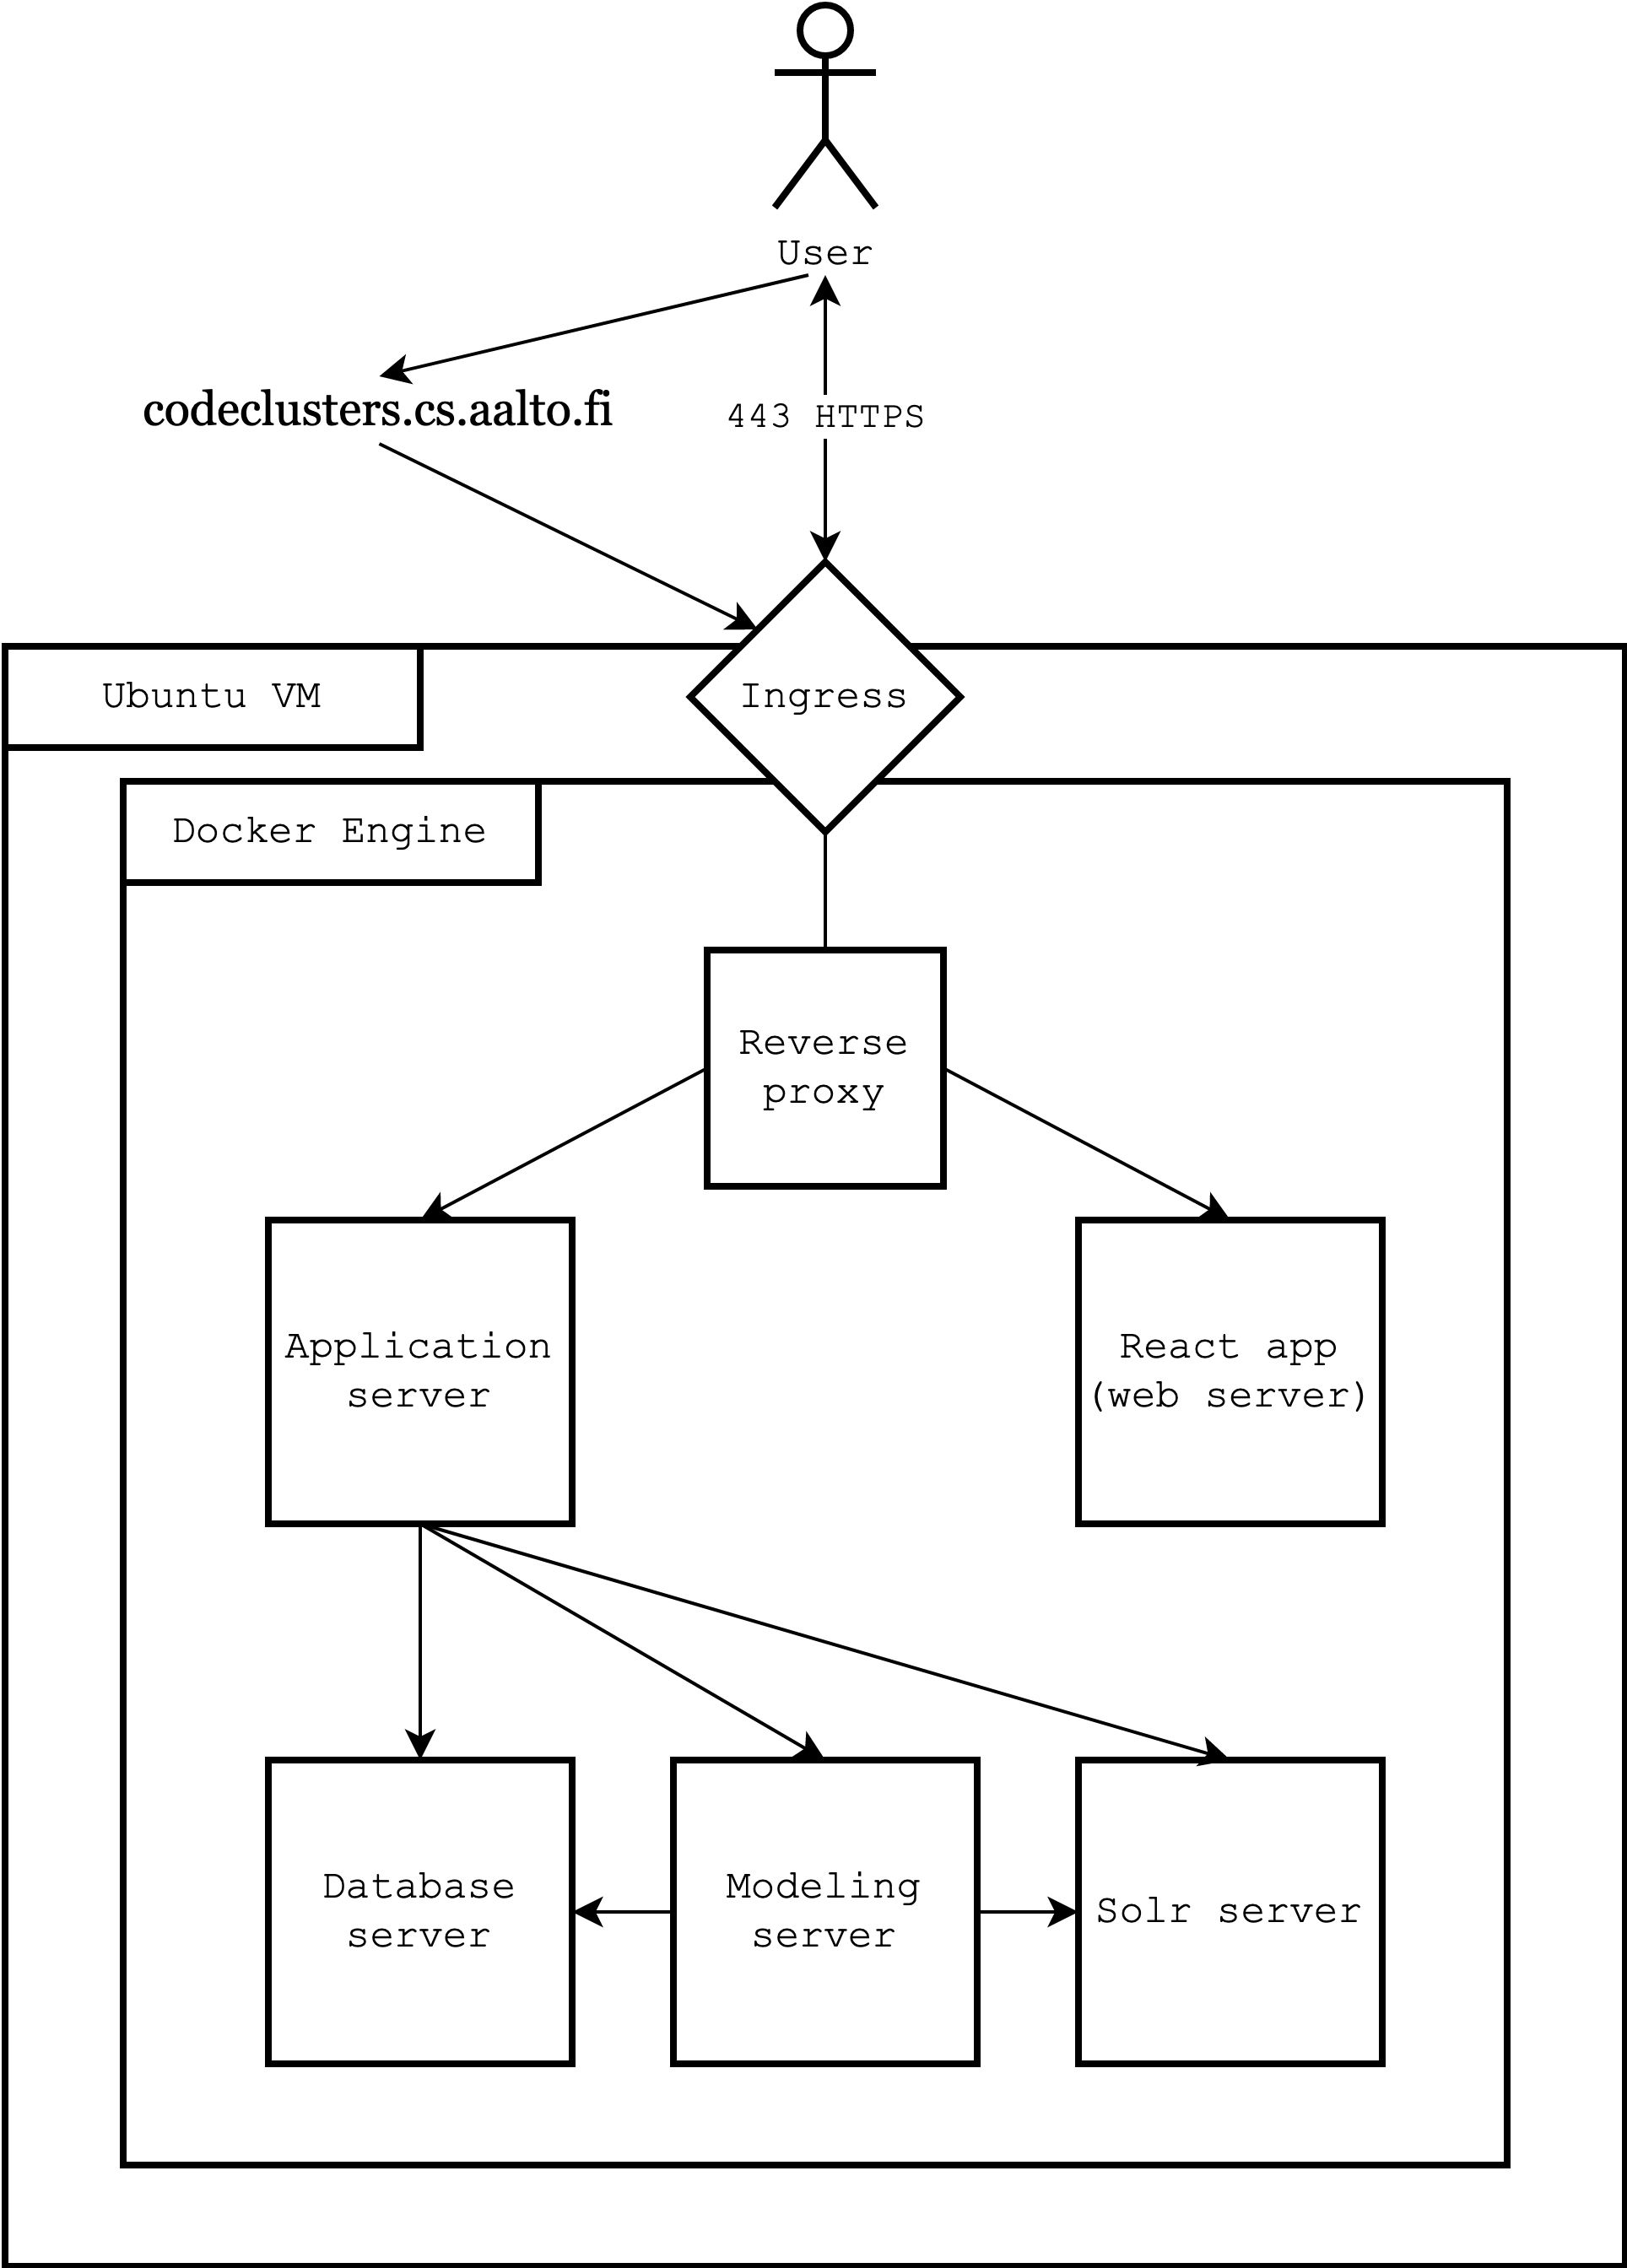
\includegraphics{images/architecture.png}
\caption{Architecture graph of the deployed Docker containers\label{fig:architecture}}
\end{figure}

At its core, CodeClusters is a web site that can be accessed with most web browsers\footnote{\url{https://codeclusters.cs.aalto.fi/}}. It is divided into 6 parts that are run as individual containers on a single Linux Ubuntu virtual machine (VM) (see Fig.~\ref{fig:architecture}). The containers are managed by Docker Compose and the server configuration written as \texttt{docker-compose.yaml} files. This simplifies the development and deployment of the system and using containers allows managing the various dependencies of the servers easily.

Majority of the system is written in TypeScript, with the application server (Node.js\footnote{\url{https://nodejs.org/en/}}) and web application (React\footnote{\url{https://reactjs.org/}}) both written in TypeScript. TypeScript is a popular language in web development that should be fairly easy to learn for anyone familiar with JavaScript. Homogenizing the server and client code enables developers to focus on one particular language, which provides also practical benefits such as sharing code between the two. Perhaps most importantly the author of this system is very familiar with the language, which made it an easy choice. Other used programming languages are HTML, Sass and Python with little snippets of Bash scripts and SQL.

\subsection{Reverse proxy}

The entry point to CodeClusters is the reverse proxy which handles all the incoming requests and forwards them to the correct services. From security standpoint this is important, as single point of entry makes it easy to manage the security and the network configuration of the website, as well as the SSL certificates. It is implemented using Nginx\footnote{\url{https://www.nginx.com/}}, a very popular web server software, due to its good performance and reliability.

\subsection{Web application}

The majority of development effort on CodeClusters was spent on the user interface (see Fig. \ref{fig:cc-frontpage} and Fig. \ref{fig:cc-modeling}), which is a single-page web application (SPA) implemented using the React UI framework. Using a framework such as React helps to organize the UI into modular components that can be composed and reused easily which is a standard practice in web development. React offers a solid structure to the application with most of the difficult parts, mainly re-rendering of the components, abstracted from the developer. It also offers the mixing of different programming languages: HTML, Sass and TypeScript, combined into single \texttt{.tsx} files to keep the code compact. There also exists a large React ecosystem of various libraries which allow the implementation of various complicated UI functionalities with minimal effort. The total amount of code written for the React UI consists of 78 components, 45 other individual files and 10,400 lines of code.

\begin{figure}
\begin{center}
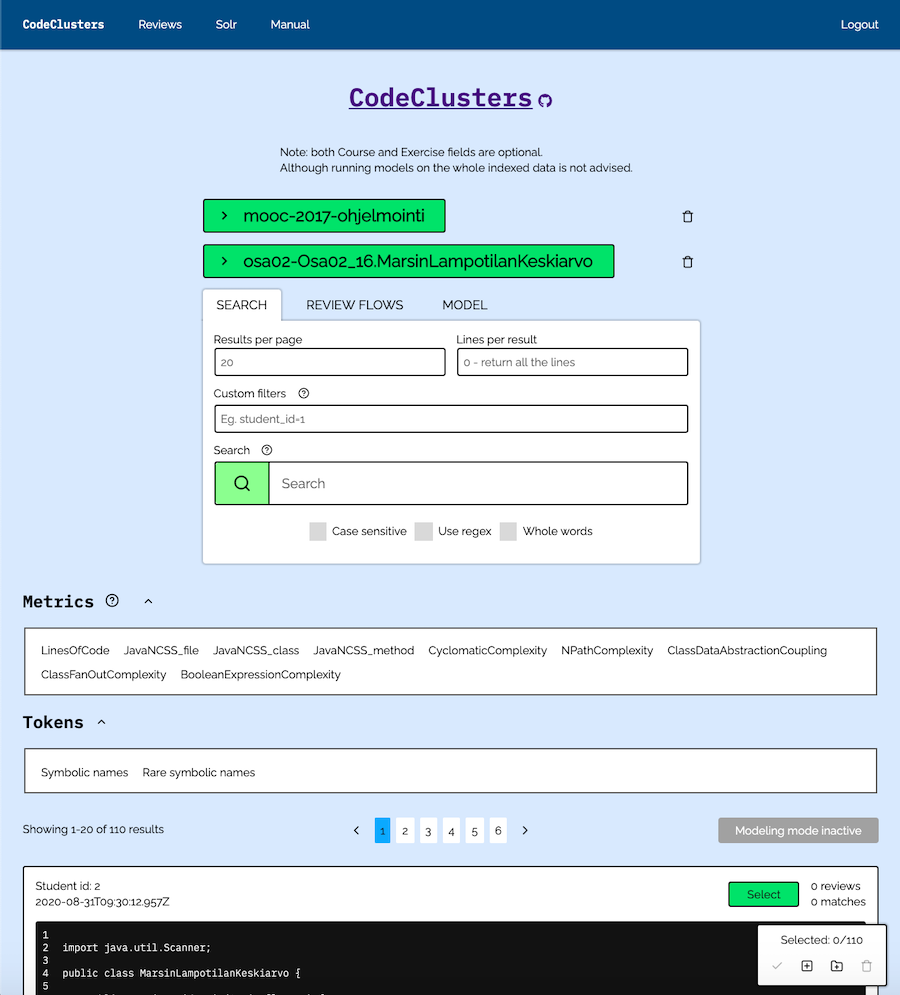
\includegraphics{images/cc-frontpage.png}
\caption{Screenshot of the frontpage of CodeClusters \label{fig:cc-frontpage}}
\end{center}
\end{figure}

The difference between SPAs and regular websites is roughly that SPAs serve the whole site as a single HTML page with the page transitions simulated to the user, whereas regular websites serve individual HTML pages for every URL address. This makes state management of the application easier as the page does not change, and SPAs also reduce the latencies between page loads when navigating the site with the overhead of having the serve the whole application at once. This, however, is a negligible issue with such a small application as CodeClusters.

\begin{figure}
\begin{center}
    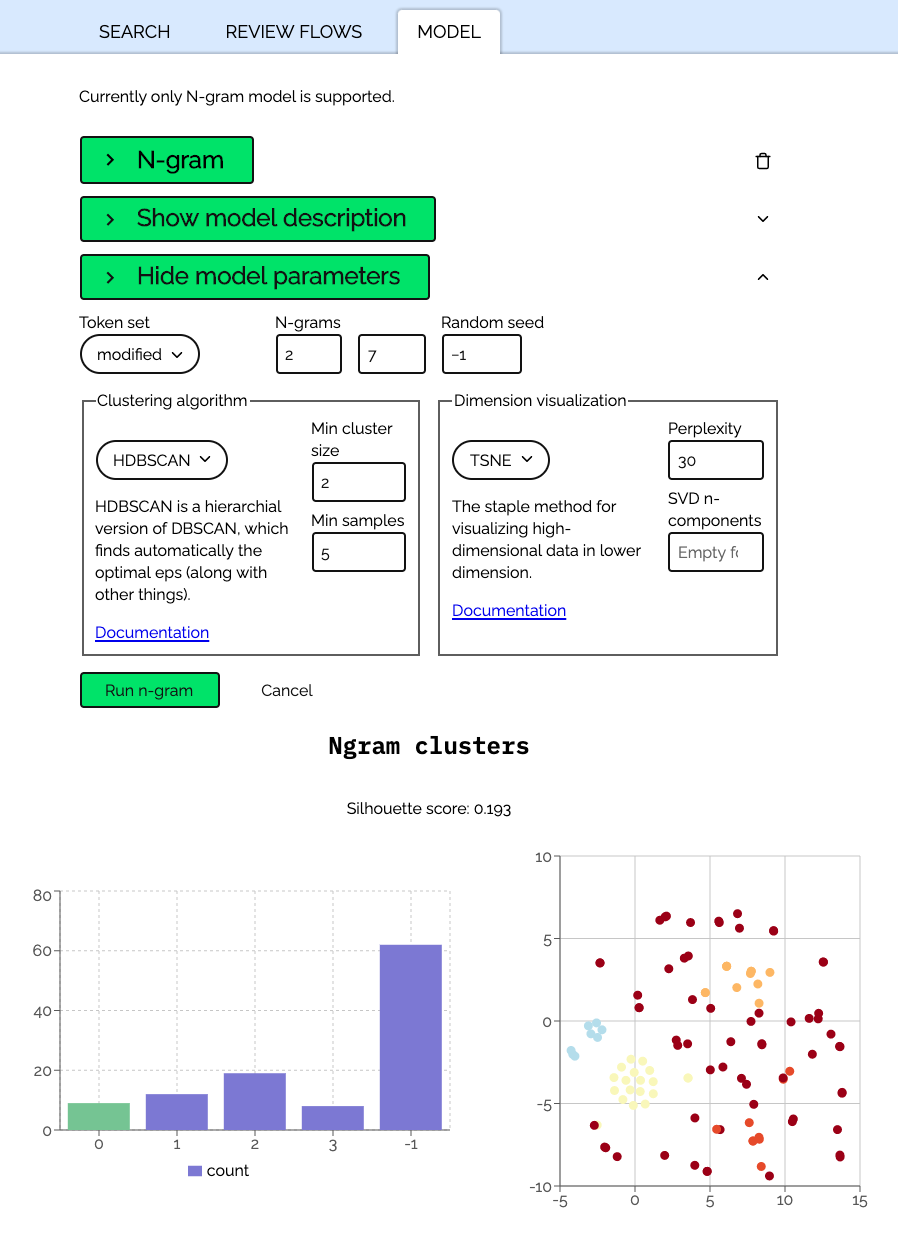
\includegraphics{images/cc-modeling.png}
    \caption{Screenshot of the n-gram model of CodeClusters. The clusters are selectable to allow reviewing of the submissions. \label{fig:cc-modeling}}
\end{center}
\end{figure}

The disadvantages of React are mainly its underlying complexity and design architecture, which requires some expertise to fully leverage and to avoid performance bottlenecks. During the development a few issues with inefficient rendering of components occurred, yet by reorganizing the components and optimizing how they updated the problems were mitigated to large extent. Otherwise, React enjoys a widespread popularity that should make future development on the UI relatively easy.

At the code level, the React code is stored in the same git repository alongside the Node.js server code. This mono-repository simplifies the management of the code between the colloquially called "backend" and "frontend", and also for example the TypeScript type definitions can be easily shared between the two. The React code is further divided into folders of components or functions that share a similar use. They follow the guideline quoted as "kitchenware principle" which means that in the same drawer, comparable to a file directory, you put the cutlery that you commonly pick up together, such as forks and knives.

\subsection{Application server}

The intermediate layer between the database, search server and modeling server is the application server, implemented as Node.js application with Express.js\footnote{\url{http://expressjs.com/}} server framework. Its main purpose is to manage the system by forwarding and composing user requests from the UI to the background services. Centralizing the application logic avoids having to control the form validation and user authentication in multiple applications, and also the separation of concerns makes the system easier to manage. Node.js\footnote{\url{https://nodejs.org/en/}} is a ubiquitous runtime environment for JavaScript that uses event-driven architecture to execute JavaScript programs in a single event loop. This has various benefits, such as simplifying the architecture by not having any threading or locking, but also drawbacks such as not being able to optimize it on as low level.

While not known as the fastest available server runtime, Node.js offers a good compromise between performance and ease of development. Given the author's familiarity with TypeScript, Node.js and Express.js, it was not deemed important to try and use other, more performant application architecture. Golang was considered but the idea quickly discarded, as the priority of the system was acknowledged to be the speed of development instead of maximal system performance. The backend TypeScript code consists of 41 files and approximately 1400 lines of code.

\subsection{Database}

It is common for web applications to use databases to store the state of the system, CodeClusters being no exception. There were no specific requirements for the database and the choice was based on the versatility and robustness of the system. In practice, PostgreSQL\footnote{\url{https://www.postgresql.org/}} was the only considered option because it was familiar to the author and widely accepted in the industry as the leading open-source relational database.

The database is accessed mainly through the application server, but the modeling server is also provided access to avoid having to pass possible large quantities of data from the application server. The database files are stored on the server's disk in a mounted Docker volume, which retains itself between server reboots.

Without specific needs other than having ACID guarantees for the data, the configuration of the PostgreSQL was left to the default settings. More important choice was, however, the choice of the database management tool to handle the migrations, querying and updates to the schemas. Instead of choosing an object-relational mapping (ORM) library that would manage everything for the developer, a more minimalistic database migration tool, Flyway, was selected. While using Flyway a lot of the database management logic of an ORM had to be programmed manually, it provided full control of the queries and the learning of SQL instead of library-specific quirks.

\subsection{Search server}

A major part of CodeClusters is its search functionality. Due to the time required to create and optimize a fully-fledged search engine, we opted for the use of an existing open-source library. The choice was then further distilled into two: Apache Solr\footnote{\url{https://lucene.apache.org/solr/}} and ElasticSearch\footnote{\url{https://www.elastic.co/elasticsearch/}}, both based on the Apache Lucene\footnote{\url{https://lucene.apache.org/}} search engine. While ElasticSearch was more popular with an extensive community and available libraries, ultimately Solr was chosen. It did not have as powerful analytics features as ElasticSearch but its focus mainly as a basic full-text search platform seemed to suit better our use case of simple code search.

The features that are indexed to Solr include the code and general metadata of the submissions such as student id and timestamp. The code is tokenized by line breaks and whitespace which creates some issues when students do not format their code properly, yet it was observed to offer the most flexibility in searching various special characters and exact patterns compared to pruning the code. Other indexed features are software metrics, generated by the Checkstyle\footnote{\url{https://checkstyle.sourceforge.io/}} static analysis library. We did not conduct a thorough analysis of the use of metrics for outlier or similarity detection and to enable the most flexibility, all of them are added to the search index. The total sums of various Java keywords are also indexed. All of these features are then searchable from the UI by either string queries that support Lucene operators, filters that specify ranges of desired values or facets, a Lucene specific feature that enables subsetting the data based on indexed values.

As all the other servers, Solr is run as its own Docker container inside the VM, with its port open for the application and modeling server. The search requests could be sent directly from the UI to the search server, but the issues with managing separate authentication service were seen burdensome, as well as the security aspects of allowing Solr to be accessed directly. We measured the latencies between sending requests through the application server and sending them directly to Solr, and did not notice major differences and thus the feature was not included.

The configuration for the Solr itself was left to minimum, most of the development time spent on creating the search queries used by the web client. For ranking the documents Solr uses Okapi BM25, a probabilistic IR model, which is the default IR model for Lucene\footnote{\url{https://lucene.apache.org/core/8\_6\_1/core/org/apache/lucene/search/package-summary.html\#scoring}}. Modifying or changing it to another model, for example TF-IDF, was not deemed necessary. The features of Solr we found the most useful are its robust search capabilities, highlighting of keyword matches and facets. 

\subsection{Modeling server}

An important goal of CodeClusters is to allow experimenting with various ways to automate and cluster the submissions, which is why the modeling server was a critical addition to the system. It was implemented using Python and Flask server framework, utilizing the scientific libraries of the Python ecosystem. It can process Java program code by either parsing it into ASTs using ANTLR\footnote{\url{https://www.antlr.org/}} parser generator or generating metrics with Checkstyle static analyzer.

\iffalse
The execution of the metrics were implemented as part of the modeling server which required it to have access to Solr and database server.
\fi

The ASTs are parsed as part of the similarity detection, for which only n-grams model was in the end implemented. TED model was also created but its slow performance made it unfeasible to use. The n-grams model allows the manual setting of various parameters such as the used set of n-grams, the used token set, clustering algorithm and the 2-D dimensionality reduction method. Most of the modeling is implemented using the basic scientific computation libraries such as numpy and scikit-learn, and the available clustering algorithms are k-means, DBSCAN, HDBSCAN and OPTICS algorithms. To plot the submissions in a two-dimensional scatter plot, a dimensionality reduction method is used with either t-SNE or UMAP algorithm.


\section{Related systems}
\label{sec:related-systems}
Various systems have been created over the years that provide analysis and clustered feedback for programming of natural language submissions. Still, no single system has become a \textit{de facto} standard for this purpose, and most systems have not seen use outside their research study setting. The following three systems presented here were chosen based on their clear architectural descriptions as well as the completeness of their implementations.

Of the three systems, OverCode has the most comprehensive documentation with all its source code public, the license however being unspecified. Codewebs's code is also public and open-sourced under MIT license but lacking documentation. Divide and Correct has perhaps the clearest architectural description but there was no open-source code found to exist. Divide and Correct is also based on natural language submissions instead of program code, but because their method for similarity detection is well-documented and applicable to code, we consider it as a valid system to review \cite{overcode, codewebs, divide-and-correct}. Next this section goes through these three systems in more detail to consider their applicability as well as possible drawbacks.

\subsection{OverCode}

OverCode~(2014)~\cite{overcode} is a code visualization and exploration tool for MOOCs, designed to help teachers and TAs to create grading rubrics or to find misconceptions, pedagogical examples and other interesting patterns. Implemented in and used for Python code, OverCode uses various static and dynamic analysis techniques to reduce the dimensionality of the submissions. As submissions are ingested by the system, OverCode executes them and by analyzing their execution graphs it discerns variables that are used similarly to rename them to one common name. It also allows creating custom rewrite-rules to merge clusters together.

The main units that teachers use in OverCode are the \textbf{stacks}, which are single lines of canonicalized code that are shown with the number of submissions they occur in. Teachers can select stacks to write feedback to the submissions, merge them with other stacks or just set them processed. A progress counter keeps track of the percentage how many submissions have been processed. Unlike other systems that use more abstract methods such as TF-IDF matrices, OverCode keeps the code very close to the original representation by pattern matching the canonicalized lines of code thus making the process very tangible to teachers.

The downside, however, of using very simple blocks to cluster the code is that OverCode might not generalize well outside the introductory MIT Python programming course it was tested on. As the exercises would become more complicated in the advanced courses, the variation between the solutions would also increase. Therefore, they might not share very similar variables that could be renamed, or lines of code that are very similar. Also, OverCode does not discern the overall structure of the code which makes it hard for the teachers to view the higher-level student approaches.

We did not attempt to replicate OverCode's functionality in CodeClusters with canonicalizing the variable names or separating them into stacks. The generalizability of the method was not deemed optimal for supporting various courses with multiple programming languages, which each would have required specific implementation for the execution graph analysis. The method also seemed hard to change or customize after its implementation. The UI choices OverCode effected the development of CodeClusters to some extent, and its simplicity was seen as an important aspect to emulate. Its available public source code was inspected yet due to its age and architecture it was not trivial to decipher, and we failed to run the application locally.

\subsection{Codewebs}
\label{ssec:codewebs}

Codewebs~(2014)~\cite{codewebs} is a homework search engine for indexing programming submissions and searching them using probabilistic information retrieval. The premise on which Codewebs is built upon is the observation that within a single, well-defined exercise the submissions contain a lot overlapping structure. By identifying the shared parts a much sparser set of decision points can be found, which defines the higher-level structure of the submissions. The teachers can then use Codewebs to find these structures to provide feedback to students on for example misconceptions or other problems.

For finding these decision points Codewebs employs various methods. At its core, Codewebs is a search engine that uses inverted index to store the submissions. All the submissions are run with a series of unit tests and their results along with the code are added to the index, both as strings and as parsed ASTs. The ASTs are not represented as graphs in the index but as linear arrays, which makes their retrieval a lot more efficient.

To retrieve documents, the user selects a seed set of \textit{code phrases} they think are semantically similar as their search query. These code phrases are subgraphs of ASTs than can be either subtrees, subforests or contexts of an AST. The user can for example select an expression \texttt{(X * theta - y)} as their query. Then, Codewebs finds the most relevant documents to that seed set by finding the exact matches of that AST as well as those that are approximately similar by a method they refer to as \textbf{semantic equivalence}.

For two submissions to be considered as semantically equivalent they need to share similar results on a portion of the unit tests. Also, the ASTs they appear in have to have a high enough probability of being submitted to the same problem. Codewebs then finds the matching ASTs subgraphs as well as the contexts they appear in, iterating over them until all the possible subgraphs and their contexts have been found that might be similar to a given seed set. For example, ASTs with a phrase \texttt{(theta' * X' - y')'} could appear in the results and teacher could provide force-multiplied feedback to all the submissions at once.

The approach Codewebs presents is quite unique with a lot of potential for further improvements. However, while they tested their system on a dataset of million submissions of Octave code, it is still questionable how well the system generalizes to other programming languages and courses. One of the main requirements they state is a large number of submissions which might not be achievable with an average MOOC course. Another constraint of Codewebs is that it is designed to work with submissions that contain a single function which is highly similar across the submissions. If, however, the exercise would be longer and the students divided their code into multiple functions, the probabilistic matching might fail to find similar AST contexts. Thirdly, the use of unit test results as part of the retrieval makes the system hard to extend to impartial exercises which do not pass the tests, and they have outlined this as possible area of future work.

To summarize, Codewebs is a highly scalable search engine to grade, analyze and provide feedback to submissions. Yet, since pursuing a similar direction would have tied CodeClusters to a specific search and similarity detection mechanism, we did not attempt to replicate their approach. Building a complete search engine in itself would have required considerable effort which would have been further inhibited by Codewebs's lack of documentation. We did not also have test results as part of our dataset, making the use of the same similarity detection method unfeasible.

\subsection{Divide and Correct}

Divide and Correct by Brooks~(2014)~\cite{divide-and-correct} is a system to read, grade and provide feedback to short answer natural language submissions at scale. It applies similarity detection by combining multiple features and transforming them into a single distance metric, after which they are clustered using k-medoids algorithm. Using a web UI the users can grade and provide feedback to the individual clusters.

The unique features of Divide and Correct include its hierarchical clustering which allows teachers to first divide the submissions into up to 10 clusters and then further divide them into maximum of 5 subclusters per cluster. By constraining the number of clusters and subclusters the complexity of the task should stay relatively stable regardless of the number of submissions. If a submission does not fit into any of the clusters, it is put into a miscellaneous cluster or subcluster.

Divide and Correct uses for its similarity detection a distance metric computed for all the pairs of submissions using length, shared words, TF-IDF term similarity, string matching and Wikipedia based LSA similarity. The clusters themselves are created with k-medoids clustering algorithm with some minor modifications. This approach is based on their previous research on a novel clustering method Powergrading \cite{basu-powergrading-2013}.

To grade and to provide feedback to the submissions teachers would choose a higher-level cluster from the UI first, whose subclusters would then automatically inherit the same grade and feedback. Teachers could then go through the subclusters and change the grade and feedback on a subcluster basis. Although not recommended, teachers could also go through the individual submissions and change their grade and feedback. This, however, would eliminate a lot of the benefits of the clustering.

The system was evaluated by comparing it to a flat grading system in which the submissions were processed one by one, their test users consisting of 25 teachers with various backgrounds and the test dataset of 2 exercises which each contained 200 submissions. The study was conducted as a within-subjects study in which the teachers used both systems for grading and providing feedback to the submissions. The first group of 10 teachers started with Divide and Correct, the other 15 with the flat grading system. A golden standard from Powergrading Corpus was used as a baseline for grades.

They found the grades to be very similar between the groups and consistent with the baseline. Using Divide and Correct, however, teachers provided a lot more feedback compared to the flat grading and the teachers also noted it made providing feedback easier. A major difference between the groups was the time it took for teachers to perform the task, using Divide and Correct teachers were able to go through the submissions roughly 3 times faster. In the post-study questionnaire majority of the teachers preferred Divide and Correct to the flat grading, 21 out of 25 considering it better. One of the complaints teachers had for Divide and Correct was the complexity of working with the clusters, as it sometimes led to a lot of rechecking and backtracking on the answers.

Divide and Correct appears as a well-rounded approach to grade, feedback and cluster natural language submissions with various similarities to CodeClusters. They both use term-based TF-IDF matrices for similarity detection, allow clustering with k-means type of algorithm and the submissions from one cluster are selectable from the UI to write feedback from one view.

Since Divide and Correct was designed for natural language text submissions instead of code, some parts of its approach are less feasible to replicate. For example, the use of the same similarity detection algorithm is unfeasible as it is tailored for natural language. Also, CodeClusters is designed to allow experimentation with multiple clustering algorithms and it could not be specialized for one type of algorithm. Using hierarchical levels for clusters and constraining their number seemed as a very interesting idea to experiment but it would have required considerable engineering effort to implement it without making the system less flexible.

While promising, Divide and Correct suffers from the same problem as OverCode in that while it produced good results with a very specific dataset, the overall solution might not be generalizable for a wide range of heterogenous datasets. The combining of multiple features into a single distance metric seems as a promising possible future enhancement to CodeClusters, which might improve its similarity detection models. Sadly, with lack of open-source code and visualizations it was hard to assess the full validity of their system and how easily their approach could have been customized for code instead of natural language text.


\chapter{Methodology}
\label{ch:methodology}
This chapter describes the design, methodology and the structure of the study. As part of this thesis we have contributed a new system, CodeClusters, which we evaluate as well as the problem we have proposed: teachers are unable to review the large quantities of submissions in programming courses. While this thesis could be described as design science research of how to design a system to analyze, cluster and provide feedback to program code submissions, this is not sufficient in itself to describe our research methods.

\textbf{Design science research (DSR)} is an information systems (IS) research methodology used primarily for designing software but also various processes and methods. In for example natural sciences the goal is to uncover universal truths about nature and environment, and in social sciences, such as psychology, from societies and individuals. In DSR the aim is to research man-made artifacts and to evaluate their novel innovations. While DSR is quite loosely defined, as the definition below shows, it provides a theoretical framework to serve as a basis for our methodology~\cite{drs-in-is, drs-drm}.

\begin{displayquote}
\label{qt:dsr}
"\textit{Design science research is a research paradigm in which a designer answers questions relevant to human problems via the creation of innovative artifacts, thereby contributing new knowledge to the body of scientific evidence. The designed artifacts are both useful and fundamental in understanding that problem}~\cite{drs-in-is}."
\end{displayquote}

\iffalse
More sensible definition would be, that the goal in DSR is either to design a new artifact or an improvement to existing artifact to provide a (impartial) solution to a problem that is better than existing artifacts in some aspects. This in contrast to artifacts whose aims is to imitate existing designs without proposing improving the current designs. A more concrete analogue could be, that DSR is the designing process of product development while routine designs are reproductions of existing designs, more akin to manufacturing. Of course, designing in abstract is just the process of proposing 
\fi

The difficulty of applying DSR are its vague formalisms that are closer to best practices than exact criteria which may differ from researcher to researcher. It has been stated~\cite{drs-in-is} that to be considered as DSR, the artifacts must propose novel innovations compared to routine designs, but from user's perspective the novelty of the artifact is auxiliary to its impact and usefulness. Unless novelty is considered to have intrinsic value on its own, one can even consider novelty redundant when measuring the benefits achieved from designing and using a tool for a task. Perhaps the difference is that in DSR the focus is to create designs that offer improvements to the existing designs whereas with routine designs the focus is to emulate or reproduce existing designs. However, this inexactness makes following DSR formally quite problematic and, therefore, our research simplifies it to large extent. Our approach can be defined as exploratory DSR analysis which main goals are to verify that the problem we have proposed exists and that the designed artifact has potential to solve that problem to varying extent\cite{drs-drm, drs-in-is}.

The stakeholders of the artifact are mainly the teachers, but also the software developers who would have to develop and maintain the artifact as well as students who would receive feedback. There are no exact requirements that the artifact must meet, although we expect the artifact as a whole to be perceived as useful from the teachers' point of view. The contributions of the artifact include its open-source code, extensive documentation, working prototype as well as various features to explore, model and provide feedback to submissions.

It has been proposed that the DSR design cycle of artifacts consists of 3 main activities. In the relevancy cycle the problems are identified and validated as well as the desired outcomes proposed for the artifact. In the design cycle a background research is conducted into the current approaches and best practices and possible solutions are outlined. In the rigor cycle a new design or an improvement on existing design is designed - an artifact - during design iterations in which it is developed until a satisfactory design is produced. After the artifact has been developed and thoroughly tested, it can be released for field testing to evaluate it in a new relevancy cycle to start the design cycle from the beginning \cite{drs-in-is}.

In the introduction chapter we identified a research problem that was based on a proposal of the thesis supervisor which was also found in the published research. We divided it into 4 research questions that each included a different aspect of the problem with the aim of researching and designing a prototype system to demonstrate a possible solution. Next, we conducted a literature review which produced a comprehensive overview of the research and systems related to the topics of the research questions. Various possible approaches were found from which we picked the most versatile and realistic options. During this process the artifact, CodeClusters, was developed whose design was influenced by the research and vice versa. And lastly, we now propose the methods to evaluate the artifact.

We conduct a user study to evaluate the existence of the problem as well as the suitability of our artifact for solving this problem. This is done as interviews with the target users of our artifact, teachers of programming courses. The sample size for our study is small, 5 teachers, to guide the design process of the next iteration of the artifact rather than to evaluate its completeness.

In addition to this study, we also use a set of user interface design criteria proposed by Gram and Cockton~\cite{drs-drm, drs-gram-cockton-1996} to evaluate our artifact from user and software engineer perspective. While the criteria are not exhaustive of every possible aspect of an UI, they help to verify how well CodeClusters satisfies the basic requirements for a software product. Other more formal evaluation criteria, such as ISO/IEC 25010:2011\footnote{\url{https://www.iso.org/standard/35733.html}} software product evaluation or ISO 9241-210:2019\footnote{\url{https://www.iso.org/standard/77520.html}} human-centric design standards, are not used since they appear unnecessarily complicated and also incur expenses.

All the participants for the study are selected from the employees of Aalto University and University of Helsinki as they would be the most likely users of the system. The interviews were conducted in the August of 2020 using Google Hangouts or Zoom, Google Docs, Google Forms and a hosted CodeClusters application\footnote{\url{https://codeclusters.cs.aalto.fi}} with the following interview structure:

\begin{enumerate}
  \item Background questionnaire
  \item Performing of tasks using CodeClusters
  \item User satisfaction and system evaluation questionnaire
\end{enumerate}

Next this chapter goes through the different parts of the interviews in more detail, but to summarize the questionnaires are simple surveys that evaluate the context of our problem as well the perceptions of the teachers regarding the artifact. The tasks are scripted scenarios that the teachers are asked to perform to evaluate how easy and intuitive the UI is to use. The interviews are also recorded, transcribed and coded to find any thematically important ideas and observations teachers say during the interviews. The questionnaires, how users performed during the tasks and the coded interviews are then aggregated into one qualitative analysis, namely thematic synthesis, to present the overall picture of the opinions of teachers regarding the problem as well as the artifact. The interview questions and the tasks are provided in the appendix.

The analysis is described in the results Chapter \ref{ch:results} which, in combination with the literature review and reviewing of related systems, are used to answer the original research questions in the discussion Chapter \ref{ch:discussion}.

\section{Structure of the interview}

The interviews could be defined as semi-structured with the interview questions, however, being given in the form of online questionnaires instead of verbally. Teachers are free to discuss the questions at any given point and to give further justifications for their answers. Also, they are asked after both questionnaires if they have something to add regarding the themes and the questions. The questionnaires should take a fairly short amount of time which is desirable as the tasks would in turn be considerably long.

\subsection{Background questionnaire}

The purpose of the background questionnaire is to ensure that the participants have indeed experience in teaching programming courses and to analyze the perceptions teachers have regarding grading and providing feedback. The questionnaire consists of 14 questions: 5 likert-scale questions with 5-levels, 3 free-form text fields, 1 multi-choice question with free-form text "Other" option and 5 single-choice questions with 5 options, one with 4. The questions are described in the Appendix \ref{appendix:questions-1}.

It is designed to be a simple questionnaire to gauge the general impressions of the teachers without requiring them to analyze their opinions in too much detail. It would seem unreasonable to inquire the teachers in much further depth than that as the topic, from prior knowledge, is expected to be unfamiliar to the teachers and no similar systems are known to be in use.

\subsection{CodeClusters tasks}

An important part of the evaluation of software is ensuring that it fulfills the basic requirements of functioning and usability by various users. CodeClusters tasks are designed to verify these requirements by simulating an imaginary task of reviewing Java programming course exercise submissions by finding outliers as well as providing feedback using similarity detection and clustering. The 110 submissions used in the tasks are solving a variation of the Rainfall Problem, which is considered as a relatively difficult exercise for beginners \cite{rainfall-2015}. The use of very scripted tasks instead of a more free-form approach allows limiting the time required to conduct the interview and it should also make the teachers feel less overwhelmed using an unfamiliar system.

The tasks are divided into 4 main parts with each part addressing a different aspect of the system and they are in order: search, modeling, review flows and reviews. To perform them, the teachers login to a hosted CodeClusters service that is seeded with the test dataset and reset between the interviews. The tasks can be found in their entirety in the Appendix \ref{appendix:cc-tasks}.

The first part of the tasks consists of searching code using the Solr search server. They require teachers to find the correct controls and to use them to perform various searches. Teachers will use various features of the Lucene API, such as facets and filters, to showcase the search capabilities of CodeClusters. 

In the second part the n-grams model is executed to create clusters of submissions. Teachers are not expected to understand the model, or its implementation, and all the parameters are provided in the task description. In the tasks they are asked to inspect the generated clusters and to compare them against each other. The goal is to see how well the teachers can process the clusters and do they find any structural patterns amongst them. The tasks should demonstrate how such the models behave in general and what are their possible shortcomings.

In the third part teachers use the review flow functionality of CodeClusters. Review flows are a unique feature of CodeClusters that allow the composition of search, modeling and review into a single executable action that would help to further automate the repetitive parts of the review process. They are asked to create a very basic review flow to demonstrate its functionality.

And lastly, the teachers are asked to test the review overview functionality which allows them to see all the submissions in a single view with the provided feedback. They are asked to edit a few of the associations between the reviews and submissions and then to accept them.

\subsection{User satisfaction and system evaluation questionnaire}

The third part of the interview is the user satisfaction and system evaluation questionnaire, which consists of 9 questions. These are 5 likert-scale questions with 5 levels, 3 free-form text fields and 1 multi-choice question with free-form text "Other" option. The questions are described in the Appendix \ref{appendix:questions-2}. The teachers are asked for their impressions regarding CodeClusters and how they would see its features, the search, modeling and reviewing, be of use for analyzing and providing feedback to course submissions.

\section{Analysis of the results}

For the analysis we combine the results of the coded transcripts of the interviews, the questionnaire answers and the performance of the teachers during the tasks. We process the questionnaires and tasks chronologically and synthesize all the related information per major topic. Any statistical methods are not used due to the low sample size and the inexactness of the measured phenomenon. We also evaluate the artifact by UI usability criteria to affirm it fulfills the basic requirements for a software product. Without statistical methods the results are hard to verify for veracity, yet they should provide a general impression to validate the problem as well as to guide the next iteration of the artifact.


\chapter{Results}
\label{ch:results}
In this chapter a qualitative analysis of the provided answers to the questionnaires, how teachers completed the tasks and about the general commentary during the interview is conducted. The small sample size of 5 is not large enough for quantitative analysis with statistical methods but it was sufficient for exploratory analysis.

To summarize, the results are mostly positive. Teachers expressed the learning of the system within the duration of the interviews challenging, which underlined a need for a good onboarding process. The features of CodeClusters were seen quite satisfactory and had it been available to the programming language they used with an integration to their LMS, everybody would have enjoyed trying it in a programming course they teach.

\section{Background questionnaire}

All the participants declared themselves to be university lecturers, as expected. Many had long careers in education and one participant explained that in the end of the 80s and the start of the 90s the grading was manual but had since transferred mostly to automatic grading. Also, another teacher explained that the programming courses were segmented into two: the regular programming courses and the project courses. The project courses do not use automatic test suites while the regular courses are heavily automated. It was also expressed that intermediary courses exist which have aspects of both.

A small source of confusion arose from the question "\textit{Grading exercises automatically is better than by hand.}" which required explicit explaining from whose perspective it should be answered. For students, automatic grading could be seen as a worse option as they would receive less personalized feedback. However, since teachers are heavily constrained by the available time to run the courses, the participants were specifically asked to consider the question from a teacher's point of view. One teacher also noted that receiving instant grades and feedback is far more useful for the students than one that is provided perhaps a week later, since students might not even bother reading it or pay much attention. Almost everyone viewed automatic grading better.

For the free-form text field questions "\textit{If you had to grade an exercise by hand, what would be your process roughly?}" and "\textit{If you had to give feedback in writing to student for an exercise, what would be your process roughly?}" the answers are highly similar, possibly because the manual grading process would also involve writing of feedback. Yet, as one teacher explained they had not even reviewed manually programming exercises and by how inexact some of the answers were, it would seem that manual grading and providing feedback is not that commonplace. The questions did not specify the type of the courses, regular or project courses, and no teacher explicitly differentiated between the two. But a good guess would be that in practice most of the time, if not always, only the project courses are manually graded and provided feedback.

The process is described in general to be the checking of the model solution, then grading and writing feedback based on the problems. Many mentioned the use of grading rubrics or checklists that would define the criteria for evaluation, such as Rubyric~\cite{aalto-rubyric-2009}. One participant also mentioned the use of Github issues and messaging applications such as Telegram for providing feedback.

Almost all participants agreed on too few teachers and teaching assistants, alongside having a large number of students, being the main problems with providing feedback to students. 

On the effectiveness of providing feedback, everyone agreed on it being very important part of learning process. Similarly, every teacher agreed that knowing how students solve an exercise is very important. The answers were dispersed, however, on the approach to check the student solutions. The majority of answers were neutral on the question "\textit{I often check student submissions to see how they have approached a problem.}" and during the interviews it was mentioned that a tool exists that provides snapshots of students' code by specified intervals, allowing teachers to see how they have progressed towards solving the exercise~\cite{hy-code-browser-2014}. However, based on the answers and what teachers mentioned during the interviews, it is evident that the final passed submissions are not collectively analyzed. Perceptions on the overall applicability on automated feedback were mostly positive, yet it was mentioned that the quality of the automated feedbacks is another matter. It took in average 5 minutes to answer the questionnaire.

\section{CodeClusters tasks}

The teachers were given an imaginary task of reviewing Java programming course submissions for outliers or other interesting patterns and to provide simulated feedback. To save time all the tasks were scripted and the teachers given help whenever it became clear that they did not know how to perform the task. It is very evident that asking people to use completely unknown system is not without drawbacks, and many of the teachers explained that they did not always understand the function of the task performed. This may also have been caused by the context of the tasks not being very discernible, which was difficult to provide given that they were simulated without prior experience using the system for programming courses.

During the search tasks, many had problems in finding the correct buttons without help as many of the buttons did not have indicative titles on their function. Shortly explaining where to look did always result in the participant finding the correct controls.

In a task where teachers used the Lucene facets, teachers were asked to select a bucket of submissions with cyclomatic complexity of 3. Only one submission existed of this kind and they were asked if they saw anything wrong with the submission. None of the teachers detected the incorrect use of BIT\_AND operator (\&) instead of AND operator (\&\&). Many of the teachers did explain that they had not used Java for a long time, but still this would indicate that teachers might be unaware of the possible erroneous ways to solve the exercise which the automated tests have failed to capture.

After using the search interface for a while, all the teachers became quite familiar with it and although some parts of the UI were less intuitive than others, for example the advanced search or modeling, the teachers did not seem to have persistent problems with the UI. However, it would require a longer time for teachers to use the system to verify this conclusively.

In the modeling tasks, teachers were asked to run the n-gram model and compare the submissions between the clusters. The model divided the submissions into structurally very similar clusters that shared the same syntactical tokens all the way to the individual ordering of the statements. The difference between two clusters might have been the use of additional variable or having \texttt{else if} instead of \texttt{if}.

The comparison, however, proved to be difficult and not many teachers were able to detect the differences without help. One teacher even mentioned that without having the submissions side by side, it was not easy to remember what they were comparing against. This underlines a need for user interface improvement to allow side-by-side comparisons.

The remaining tasks teachers performed without major problems although the layout of the submission-to-review grid was a bit non-obvious to the teachers. They did not immediately see that the rows are the submissions and the columns the reviews, and the behaviour of the linking and unlinking of reviews was not completely clear.

In total, the time it took to perform the tasks ranged from 30 to 50 minutes, depending on how much the teacher wanted to discuss the system and analyze the submissions.

\section{User satisfaction and system evaluation questionnaire}

For the first question, the majority of answers were neutral on CodeClusters being easy to use. This correlates with how the teachers performed the tasks and which highlights a need for a good onboarding process and UI improvements. There also exists inherent complexity in using the full Lucene API and setting the modeling parameters manually, which probably contributed to the overall impression of complexity. Majority of the teachers chose as the main problems with CodeClusters the unfamiliarity and the unintuitivity of the UI.

For improvements most wrote only one, although the answers were unique across the participants. Many said during the interviews that they would like to use the system with a programming language their course used. Also some noted that they wanted a better way to compare submissions from different clusters and from even different searches or differently parametrized models. One feedback asked for moving the search closer to the results.

A majority agreed on the code search being useful in finding interesting submissions, although a portion was neutral on its applicability. On the modeling part there was a similar split where the majority agreed that modeling could be useful given future improvements, a portion being neutral. Everybody agreed sending feedback is useful with the split being half on "I agree" and "I strongly agree".

On the problems of giving clustered feedback the majority of teachers, either directly or indirectly, were suspecting of the applicability and reliability of the clusters. Similarly, the tuning of the model and setting its parameters were seen hard to grasp. The user interface was also expressed to could have been better.

For the question "\textit{What did you like the best about CodeClusters? Would you consider using it given improvements?}" all the teachers expressed interest in trying it for a programming course they teach. Many saw it having a good potential in being a helpful tool for analyzing large quantities of submissions that otherwise would go unprocessed. Everybody agreed and majority of them strongly, that they could see providing additional feedback being implemented to programming courses with a system similar to CodeClusters. The second questionnaire took in average two minutes to answer.

\section{Criteria-based evaluation}

We evaluate our artifact for basic software product requirements it should meet using the UI design criteria proposed by Gram and Cockton ~\cite{drs-drm, drs-gram-cockton-1996}. They categorize these requirements based on the stakeholder, user or software engineer, as well as on properties which the UI or the system around it should satisfy.

\bigskip
\noindent
From \textbf{user's perspective}, in our case teachers, the criteria are as following:

\begin{enumerate}
    \item \textit{Goal and task completeness: you can do what you thought of doing}
    \item \textit{Flexibility: you can do things in several ways}
    \item \textit{Robustness: you can avoid doing things you wish you had not done}
    \item \textit{Learnability: the ease with which novice users can acquire competent performance}
    \item \textit{User satisfaction: how a system makes users feel in terms of sense of achievement or excitement}
\end{enumerate}

For the first criteria, the artifact can be considered to have average goal and task completeness. While the tasks were scripted, on many occasions teachers did not always find the proper UI controls or understand how they behaved. This could also be contributed to common unfamiliarity which is universal to all UIs.

CodeClusters has moderate to high flexibility as many of the operations can be done in multiple ways. The search supports using various parameters to receive the same results and feedback can be added with clicking the submissions or using the small menu at the bottom right corner. The n-gram model also enables flexible parametrization which supports various clustering algorithms and token sets. Using review flows the different operations can also be composed into single executable actions.

Robustness of the artifact can be considered as moderate to high. All the actions can be reversed without permanently modifying the state of the system and there are edit or delete controls for majority of the database schemas. The UI is quite explicit in its behavior and although some operations, such as manually selecting submissions and then resetting them with the bottom-right menu, are possible, doing that by accident should not a consistent problem.

Based on the second questionnaire and the task performance, the learnability of the artifact is probably low to average. Some teachers were able to grasp the UI better than others, yet some would have not been able to use it without exact instructions. In time perhaps the user could acquire solid understanding of the UI but it is difficult to extrapolate this based on our results.

User satisfaction of the artifact is not very easy to assess on such short timespan performing the tasks. While most of the teachers were neutral on CodeCluster's ease of use, everyone also agreed that the artifact would be interesting to use in a programming course they teach. Teachers did seem to appreciate the features of CodeClusters, the speed it executed operations such as search or models and the overall objectives of its design, but to conclude how satisfied they are would require actual user experiences using it in programming courses. Therefore, at this stage of the artifact, an estimation of moderate user satisfaction is perhaps the most accurate.

\bigskip

\noindent
From \textbf{software engineer's} perspective the design criteria are~\cite{drs-drm, drs-gram-cockton-1996}:

\begin{enumerate}
    \item \textit{Modifiability: how easy it is to modify the system when facilities have to be extended}
    \item \textit{Portability: how easy it is to change its hardware and software environments}
    \item \textit{Evaluability: how easy it is to evaluate the system against quality goals}
    \item \textit{Maintainability: once installed in an environment, how easy it is to maintain the system}
    \item \textit{Run-time efficiency: whether the system consumes an acceptably low fraction of computer resources}
    \item \textit{User-interface integratability: how easy is it to integrate the interactive system with existing or new software applications}
    \item \textit{Functional completeness: whether the system has sufficient functionality to support users to do their tasks}
    \item \textit{Development efficiency: whether the most effective use of resources is being made during system development}
\end{enumerate}

The system is written in popular programming languages such as TypeScript and Python and it uses popular libraries and frameworks such as React and Solr. Also, while the system lacks tests it has been built to meet the quality requirements based on the author's experience working as a software developer in the industry. This should make the adding of future modifications convenient given that the developer has experience working with these technologies. Therefore, the modifiability of the system should be moderate to high.

Using Docker containers the different parts of the system are insulated from conflicting dependencies which keeps also the build process very reproducible. Any environments that support Docker and Docker Engine should be able to run the system, although the deployment and other scripts are written in Bash which are not portable to all operating systems. The portability of the system can therefore be seen as very high.

We have not specified any quality goals the system should meet which makes assessing its evaluability somewhat difficult. All the code has been produced to the level of quality standard of the author, which might be seen as above average. The clear separation of concerns of the system as well as code, can be considered to follow the best practices of architecting software. Every part of the deployment and running the system locally are documented, which was a purposeful aim during the development. The evaluability could therefore be seen as moderate.

The maintainability of the system would be high from both deployment and development perspective. Once the application is deployed, it should stay running without problems and restart gracefully. To deploy new versions the process is well-documented albeit manual. From development perspective the system is also easy to run locally and most parts are executed as Docker containers.

Run-time efficiency of the system is high, although there definitely are bottlenecks in the processing pipelines that might become restricting with large datasets. The search and UI uses pagination to limit the number of shown and processed submissions, but the execution of models and the submission-to-review grid require fetching of all the submissions to function. The Solr server takes the majority of RAM of the system with the other services, such as Nginx and Node.js, taking only negligible amounts.

UI integratability of the system is average to low, depending on the evaluation criteria. Certainly CodeClusters should have an integration to at least one LMS with university credential-based user authentication. However, as a separate service CodeClusters is easy to add to existing systems and it does not conflict with previous workflows.

Functional completeness of the system is still low although a lot of features have been implemented to varying extent. The search functionality of the system is quite complete, but the modeling and review parts still require additional work as well as the integrations to other systems. All the features also require testing by the teachers to process actual course data and proper integration and unit tests.

Development efficiency of the system at its current stage is average to high, depending on the skill set of the developer. Most of the major architectural choices have already been made and the configuration, as well as the boilerplate, written to large extent. Therefore, any new developers could spend their time on the actual features instead of unrelated tasks.


\chapter{Discussion}
\label{ch:discussion}
This chapter discusses the results of the interviews, as well the findings of the background research and the design of CodeClusters. We synthesize them in the context of the original research questions and evaluate how sufficiently we are able to answer them.

\section{Answering the research questions}

As stated in the introduction chapter, the subject of this thesis has been the many facets of reviewing and providing feedback to large quantities of submissions in programming courses. This topic was divided into four research questions that each address a different part of the problem. Through literature review in Chapter \ref{ch:background}, building a new system as described in Chapter \ref{ch:system-description}, reviewing of related systems in Section \ref{sec:related-systems} and our study, we have gathered a solid understanding about of the context of our problem as well the practicalities involved in solving it.

\bigskip
\noindent
\textbf{RQ1: How code can be represented for efficient search and modeling?}
\bigskip

\noindent
There are a multitude of options to represent code which each suit different purposes. We discussed the basics of information retrieval and search in Section \ref{sec:ir} in which we used arrays to represent text or code. Since search involves mostly text or other unstructured data, an array is an efficient solution to process and query large quantities of documents. Parsing the text into tokens and transforming them into vectors of a vector space model allowed the use of TF-IDF matrices which are flexible yet not always accurate representations of documents.

But in contrast to natural language text, our documents are program code which follow a very strict grammar and hierarchy that allow compilers to parse and execute them. AST is perhaps the most well-known intermediary representation which represents the full hierarchical form of the program which can also be represented as a graph. Another common form is the CFG which represents the execution paths of the program. For search, graphs may not be very sufficient to use as such but as demonstrated by Codewebs, the hierarchical form of the graphs can be leveraged to find subtrees or contexts of ASTs\cite{codewebs}.

For modeling, arrays as well as graphs are both suitable although graphs heavily restrict the available algorithms. Quantifying the code into numeric values, metrics, makes it easy to process, although their applicability for discerning structure or other deep phenomenon is lacking. In outlier detection they might be useful as any values over or below average might reveal unique solutions to the exercise, which using CodeClusters and cyclomatic complexity seemed to find unusual submissions. The main focus of the models in this thesis has been similarity detection to find structural similarities to provide clustered feedback to multiple submissions at once. For that purpose, graphs or arrays were the most common representations found in the related research\cite{fox-clust-leverage-2015, fox-roy-autostyle-msc-2016, codewebs, divide-and-correct, glassman-reusable-feedback}.

TED\cite{zhang-et-al-1989} is a popular graph algorithm for code similarity detection which generates a matrix of edit-distances for a set of graphs. It is, however, very expensive to run with a worst-case complexity of approximately $O(n^3)$ \cite{ted-demaine}. For similarity detection of submissions, Fox et al. noted that a weighted version of TED produced more reliable results than the basic version, although there was no mention of the execution time for their 800 Python submissions \cite{fox-clust-leverage-2015}. In small scale, weighted TED might be suitable although the experience with CodeClusters showed that the implementation should be carefully crafted to achieve fast execution times utilizing perhaps multi-threaded processing.

As an alternative, arrays are a lot more efficient to process and they can be easily scaled to large datasets as demonstrated by Codewebs with a dataset of million submissions \cite{codewebs}. To score similarities between arrays, GST\cite{wise-gst-1993} could be used yet as the experiments with TED showed, its high worst-case complexity and poor ability to find higher-level structures might make it non-optimal. The major problem of arrays is that they lose the original structure of the AST or CFG.

Generating n-grams of the token arrays would retain some of the structure of the original graphs. These could be generated sequentially, or as proposed by Karnalim and Simon~\cite{simon-better-ngrams-2020}, hierarchically from the AST. This could improve the detection of higher-level structures in the code. Similarly using CFGs or a combination of CFGs and ASTs might improve the detection of higher-level patterns \cite{cfast}. Tuning the used set of tokens might produce better results which were experimented with CodeClusters\cite{jplag, wahlroos-2019}. The used model in CodeClusters also used ranges of n-grams that seemed to generate more balanced results compared to a single value of $n$.

These n-grams could be transformed into a vector space model, similar to search, and use cosine similarity and dimensionality reduction to improve the results. As TF-IDF matrices, however, the arrays would also lose their sequential order in addition to losing the hierarchical structure of the graphs. Generating n-grams instead of single tokens might mitigate this to some extent, yet arrays cannot fully replace the original graphs. Combining the n-grams with other features could be incorporated in the model, as demonstrated by Divide and Correct~\cite{divide-and-correct}. There might exist NLP methods for text that could be applicable to code as well.

\bigskip
\noindent
\textbf{RQ2: What methods can be used to analyze and cluster code?}
\bigskip

\noindent
The literature review provides a multitude of possible approaches to analyze as well as to cluster code. For the analysis, we categorized the approaches in the Section \ref{sec:analyzing-code} as either manual or programmatic review. The manual reviewing might be very monotonic and time-consuming and it is what thesis aims to avoid by designing a novel approach and system. Yet, it could be worthwhile to manually review some of the student submissions to understand how to automate the process \cite{glass-feature-engineering, rogers-auto-style-2014, luxton-sub-variation-2013}.

For programmatic review, we mostly discussed static analysis to analyze the submissions with pattern-based matching to reveal problems in the code and to provide feedback messages. A popular static analyzer is the linter\cite{lint-1988}, which evaluates stylistic and quality aspects of the code. Static analysis might provide very extensive information about latent errors in the programs which are not immediately obvious to developers, and they are very popular in the software development industry \cite{fb-static-dynamic-analysis}.

Using a similar static analyzer in programming courses might not, however, be as desirable as students could find it hard to follow the advice of the analyzers as well as to complete the exercise. Requiring the same level of rigour from students as from software engineers might be unwarranted. Also, the students might have not been even instructed on quality concepts during the course\cite{crow-code-quality-2020}. Static analyzers have been customized for pedagogical purposes in some cases\cite{static-analyses-in-py-courses}. The effort required to customize a static analyzer might be substantial and be seen as very similar to creating additional automated tests. Executing the static analyzers after students have solved an exercise would seem non-optimal as the students would probably not be engaged with the problem anymore and thus not interested in internalizing the feedback very deeply. To fully understand their applicability, additional research is required into how to implement them, how the students react to them and do they improve the students' learning or quality of the students' code.

Another approach for automatic code analysis could be the intelligent tutoring system (ITS), which generates more holistic feedback messages based on extensive student data. They are designed to simulate personalized tutoring assistance and provide help proactively during the students' solving process. Glassman et al. demonstrate MistakeBrowser and FixPropagator to analyze failed student solutions and to find the minimal number of transformations to fix them. With the systems, teachers can provide tailored feedback to all the students on the same problem\cite{glassman-reusable-feedback}. An ITS could provide advice whenever a student was unable to progress, writing unnecessarily complex or inefficient code, or in general when they wanted to receive advice. This could help in preventing students from developing bad programming habits. The implementation of an ITS would, however, require substantial effort and expertise \cite{glass-feature-engineering, its-2020}. 

The similarity detection methods produce either similarity or distance matrices, which we would want to cluster into meaningful groups for the teachers to use them for providing force-multiplied feedback. For this purpose, many of the staple clustering algorithms seem sufficient. Depending on the data, however, some of the algorithms might be less optimal to use since they have different preconditions how they expect the data to be distributed.

K-means algorithm would be suitable if the data was globular and easily partionable or if the teacher wanted to use a predefined number of clusters. DBSCAN would be a better choice for more asymmetric data that had clear dense regions surrounded by lower-density boundary regions. Yet as DBSCAN might not cluster well data of varying density, OPTICS or HDBSCAN might suit the task better. It is difficult to evaluate the optimal algorithm when the data might vary considerably between exercises or programming languages.

However, as demonstrated by Fox et al.~\cite{fox-clust-leverage-2015} and through experimentations with CodeClusters, a density-based clustering algorithm might be the most versatile approach for very heterogeneous data. Algorithms such as OPTICS or HDBSCAN are robust to varying density and they do not require a high level of expertise to set their parameters. But it should be noted that poor quality data would be impossible to cluster well regardless of the chosen clustering algorithm.

\bigskip
\noindent
\textbf{RQ3: How code submissions can be reviewed and explored efficiently?}
\bigskip

\noindent
If the baseline of reviewing and exploring submissions is going through them one by one to grade, provide feedback or to analyze them for patterns, there are various problems with this approach. With a high number of submissions this process is very time-consuming, susceptible to biases between different teachers, repetitive and inflexible in case the evaluation criteria is altered during the process. A grading rubric might help to maintain consistent evaluation criteria but it does not help to reduce the burden of the task. A solution could be to completely automatize the task by creating a static analyzer, which would discern the code with pattern matching to find various structures that could be used as indicators of possible problems.

However, creating these patterns with proper feedback is lacking in sophistication and it can in turn be as or more tedious as going through the submissions one by one. Also, many analyzers are not suited for pedagogical purposes and they work on individual programs, not on collections of similar code. Rather than attempting to manually define all the possible criteria how to review the submissions, a more flexible approach could be to reduce the dimensionality of the original data and letting teachers to be in control of the reviewing of the clusters. Reducing the code into numerical values, metrics, has been a subject of research since the 1970s but their use as for example indicators of complexity is hard to justify\cite{halstead-1972, mccabe-1976, cc-is-loc, shepperd-cc-1988}. Instead, using a similarity detection method the code could be discerned for similar structures which the teachers could evaluate and use for providing feedback. By receiving an overview of the higher-level structural approaches, the teachers might also gain a more in-depth understanding of the submissions while making the task quicker and more efficient than manual review.

For the detection of similarities various representations of program code could be used. For example ASTs contain the full hierarchical structure of the programs, CFGs the execution flow and token arrays the individual syntactical tokens, which can be enhanced by encoding the structure into tokens or using n-grams. Their similarities can then be scored with for example TED, GST or cosine similarity using vector space model. The optimal method would have to be quick even with thousands of submissions and also be able to detect varying levels of similarity. It has been suggested that the levels of similarity could be based on structural, syntactical and presentational levels\cite{luxton-sub-variation-2013}, yet additional research is required to verify how these could be utilized in the implementation of similarity detection models.

Various related systems or approaches have also been proposed to solve this very same problem. OverCode uses stacks\cite{overcode}, Codewebs semantic equivalence\cite{codewebs}, Divide and Correct custom distance metric\cite{divide-and-correct} and Fox et al. weighted TED\cite{fox-clust-leverage-2015}. While all of their approaches are very different, they share a common goal of reducing the dimensionality of the original data by clustering the submissions based on their similarities. All of the systems could be used as a basis for a new system and their approach improved, yet their undocumented or non-existent open-source code makes them hard to utilize.

Therefore, we contributed a new system, CodeClusters, which demonstrates a novel approach to review the submissions to understand how students have solved the exercises and to provide feedback. The features of the system include a search engine in the form of Apache Solr, which can be used for ad hoc search queries that should scale even to the largest of datasets, and a similarity detection model that generates n-grams of ASTs that are transformed into a TF-IDF matrix. Using the n-grams model teachers can cluster the code into structurally distinct cluster to analyze them or to provide feedback. CodeClusters also implements review flows, a data structure to automatize the search and modeling steps with default feedback message, as well as submission-to-review grid to provide an overview to detect which submissions have received what feedback. Further research is, however, required to confirm that this approach does indeed make the task of reviewing submissions more efficient than manual reviewing. Based on the experiences using CodeClusters and on related research, the approach should have distinct advantages especially for helping teachers to gauge general student programming patterns and solution schemas in a short amount of time.

\bigskip
\noindent
\textbf{RQ4: What are the main benefits and drawbacks of CodeClusters?}
\bigskip

\noindent
From the software engineering perspective, CodeClusters meets modern software engineering standards which makes it a great groundwork for additional improvements. Its open-source codebase is clear and well-documented, the deployment process is reproducible, and it uses various popular technologies such as React, Node.js, Postgres and Docker which should make new developers feel comfortable to commence further development.

From the teacher's point of view, CodeClusters offers exciting opportunities to improve their knowledge of the student programming patterns, to provide more personal feedback to students and to improve the test suites as well as course material. Its search functionality is based on Apache Solr, a popular and robust search server which allows the use of filters, facets and Lucene search syntax. Teachers can, for example, filter the submissions by a specific range of metric values to find outliers in which the students have possibly misunderstood a programming concept. The n-grams model CodeClusters implements executes quickly and it supports various parameters.

However, during the experimentation it became obvious that the implemented n-grams model is more suited for finding very similar submissions rather than higher-level approaches. With the test dataset, it clusters the submissions based on minor differences of syntax such as the use of integers instead of doubles or \texttt{if} instead of \texttt{else if}. Also, the model can be complicated to use as it allows the tuning of various parameters that require some expertise to set appropriately. Review flows are a unique CodeClusters feature to allow composition of search, modeling and feedback messages as single executable actions, yet which require additional software development to complete their functionality. The submission-to-review grid provides an easy way to visualize the submissions and the reviews they have received.

CodeClusters was tested with a considerably small test dataset, 110 Java submissions, on which it performed efficiently. However, it is possible that bottlenecks exist that would make operations such as running the n-grams model slow although this was not investigated by using a larger dataset. The scaling of the system should otherwise be relatively easy, as increasing the number of the server instances should be enough to increase the system's capacity to process requests. Showing large numbers of submissions in the UI was noticed to cause latencies with the rendering of React components.

Although the system is more of a prototype than complete system, the first impressions of teachers were positive regarding CodeClusters but to verify its applicability in full, further development and research is needed. One design goal for CodeClusters is flexibility so that instead of a one fixed approach, teachers could compose different approaches such as search queries and models. This should provide the teachers freedom to experiment, analyze and automate different workflows to efficiently review and explore the submissions. 

Related systems and research have shown that the analyzing and providing force-multiplied feedback with a clustering approach can work to help teachers process vast amounts of program code submissions. Providing feedback during the solving of the exercise would be preferred compared to one that is given later, and perhaps an approach different from CodeClusters' would be needed to provide feedback. Nevertheless, CodeClusters allows teachers to analyze and search the submissions with a straightforward user interface which, by far and large, is not possible with the current systems.

\section{Limitations of the study}

The major problem of the study is its low sample size that cannot be considered as a comprehensive representative of the whole population of programming course teachers. Also, since the interviews did not go into too much detail of the applicability of the CodeClusters nor teachers could use it with the programming courses they teach, this limits the extent what can be interpreted from the results. While every teacher thought the artifact and the idea to be interesting and worthwhile to investigate, the study did not produce conclusive data on how the search or modeling functionality would help teachers. For confirming the problem and guiding the next design direction of the artifact the study is sufficient, yet more development and research is required to verify the artifact and its approach.

\section{Future work}

We have found many possible areas of future work regarding CodeClusters and research. Adding integrations to LMSs would be necessary to trial it on programming courses and the UI could be improved. Allowing side-by-side comparisons between clusters would be important but also a visualization to show the submissions in a more compact form. As of now, even with moderately sized clusters teachers would still have to go through a considerable number of submissions individually to discern the underlying structural patterns of a cluster. Perhaps showing a structural skeleton of the submissions, a CFG perhaps, could be a one approach, or collapsing the code by similar segments and showing only where they differ, akin to a \texttt{diff} tool.

It might be a good idea to research further how to develop a similarity detection model that is especially tailored for detecting program code similarities of varying levels. Vector space model that uses various features instead of just AST tokens and n-grams might work, yet conducting manual review first might be necessary to understand how the teachers would even prefer the submissions to be clustered. The improvements to the n-grams model could include generating the n-grams hierarchically instead of sequentially, tuning the set of used tokens and using both AST and CFG graphs. After developing the model to a high enough accuracy, it could be simplified in the UI so that the teachers could achieve good results without having to tune the parameters of the model. This would allow them to focus on the analysis of the clusters rather than on the data science of the models.

Other interesting areas include designing a system that provides more integrated feedback than one that is sent after students have solved the exercise. Students would probably find it more motivating to have the system work during their solving process rather than after it, which would require a different approach for providing feedback as proposed by CodeClusters. The benefits of adding a static analyzer might be good to study to understand if the students' comprehension and ability to write good quality code increases. Developing an ITS might be the ultimate approach for providing students with holistic and versatile feedback, yet it requires considerable effort to implement properly.


\chapter{Conclusions}
\label{ch:conclusions}
This thesis has researched how to review large numbers of program code submissions more efficiently than manually reviewing them. As an additional contribution, a new system was developed, CodeClusters, that implements some of the researched methods and which aims to offer an approach for teachers to analyze, explore and provide feedback to student submissions. The system, the problem and the ideas of using search or modeling to analyze the submissions were studied as interviews with teachers who had experience in teaching programming courses. The results of the questionnaires, performed tasks with the system as well as the overall commentary during the interviews were analyzed and discussed in the context of the research questions. The system was also evaluated for UI and system design criteria.

The results indicate that the teachers do not have similar existing systems to analyze the submissions and that the designed system would allow novel opportunities for deepening teachers' knowledge about the student programming patterns. All the interviewed teachers expressed interest in using the system with programming courses they teach, and the overall impressions were positive. Therefore, the system seems to have achieved its goal of being potentially very useful to the teachers. However, further software development and research is needed to improve the system and the proposed similarity detection model.

CodeClusters in itself is a well-documented and working prototype, developed with popular technologies and libraries such as Docker, Node.js, React, TypeScript, Python, Postgres, Nginx and Solr. It offers a robust groundwork for further development and while it became evident during the interviews that some UI enhancements are required to improve its usability, namely side-by-side comparisons between clusters, the basic approach it implements appears suitable. The search was found to be a good general tool for finding outliers that would scale well to large datasets. The implemented similarity detection model, n-grams, while producing interesting clusters, still requires improvements to better discern higher-level patterns.

Using more features in the model such as CFGs, hierarchically generated n-grams or metrics, could result in improved accuracy in detecting meaningful structural patterns yet this is left as possible future work. Developing the model to detect similarities of different levels might be worthwhile to investigate. Additionally, the system requires alongside the UI enhancements integrations to LMSs as well as support for more programming languages to be used by teachers in programming courses.

Possible applications of this research and system could improve the teachers' overall ability to understand their students' behavior better, as well as improving the learning of students and course material. Analyzing the submissions could help teachers to discern misconceptions, errors in the test suites, anti-patterns and solution schemas students have used. Providing feedback with the system might also be useful, yet sending the feedback after the student submitted their work might not be perceived by students as very relevant. The in-depth knowledge of the student behavior discovered by using a system such as CodeClusters could be used to develop better analysis and feedback systems, such as intelligent tutoring systems, that could provide more holistic feedback as the students are solving the exercises.

\iffalse
The long-term benefits from analyzing the student submissions on a high abstraction level could provide teachers with a more realistic intuition how the exercises are being solved. Combining the system with for example snap-shot based solution progress analysis could allow teachers to precisely find and understand how students flail in the exercises. solve the exercises?
\fi

 
% STEP 5:
% Uncomment the following lines and set your .bib file and desired bibliography style
% to make a bibliography with BibTeX.
% Alternatively you can use the thebibliography environment if you want to add all
% references by hand.

\cleardoublepage %fixes the position of bibliography in bookmarks
\phantomsection

\addcontentsline{toc}{chapter}{\bibname} % This lines adds the bibliography to the ToC
\bibliographystyle{abbrv} % numbering alphabetic order
\bibliography{bibliography}

\begin{appendices}
\myappendixtitle

\chapter{Background questionnaire}
\label{appendix:questions-1}

\begin{lstlisting}
Q1: Your background profession
1) Lecturer / teacher / professor
2) Computer science or software engineering student
3) Software developer
4) Teaching assistant (TA)
5) Other

Q2: How many programming courses (count each instance) you estimate you've roughly taught or been part of teaching? (even as TA)
1) None
2) <10
3) 10-50
4) >50

Q3: Over how many years these courses have roughly been taught?
1) <5
2) 5-10
3) 11-20
4) >20

Q4: During those courses, exercises were in majority of cases graded ...
1) Only by hand
2) Mostly by hand, some automatic grading
3) About equally by hand and automatically
4) Mostly automatic grading, some by hand
5) Only automatic grading

Q5: During those courses in most cases feedback was given to students in the exercises.
1) Yes, verbally
2) Yes, in writing
3) Yes, verbally and in writing
4) Yes, using automatic feedback system
5) Feedback wasn't in majority of time given to students

Q6: Grading exercises automatically is better than by hand.
1) I agree strongly
2) I agree
3) Neutral
4) I disagree
5) I disagree strongly

Q7: If you had to grade an exercise by hand, what would be your process roughly?
<free-form text field>

Q8: What are the biggest problems of giving feedback to students?
[1] Too few teachers / TAs
[2] Too many students
[3] Not possible in the current system (eg because of automated grading)
[4] Too difficult to invent good feedback
[5] Too low impact
[6] Too many exercises
[7] <free-form text field>

Q9: If you had to give feedback in writing to many students, do you think there would be a lot of repetitive work? Are there ways you would try to speed up the process? 
<free-form text field>

Q10: Giving feedback to students has no positive impact on their performance.
1) I agree strongly
2) I agree
3) Neutral
4) I disagree
5) I disagree strongly

Q11: It is very important to me to know how students have solved an exercise I have made.
1) I agree strongly
2) I agree
3) Neutral
4) I disagree
5) I disagree strongly

Q12: I often check student submissions to see how they have approached a problem.
1) I agree strongly
2) I agree
3) Neutral
4) I disagree
5) I disagree strongly

Q13: Giving good feedback can't be automated or it is too difficult to do so.
1) I agree strongly
2) I agree
3) Neutral
4) I disagree
5) I disagree strongly
\end{lstlisting}

\chapter{CodeClusters tasks}
\label{appendix:cc-tasks}

\begin{lstlisting}
Go to https://codeclusters.cs.aalto.fi

Task 0:
Login as a teacher. Select the course mooc-2017-ohjelmointi and exercise MarsinLampotilanKeskiarvo.

Task 1.0:
Search code with the word "luku". How many submissions do you find? How about using fuzzy search with edit distance of 2: "luku~2"?

Task 1.1:
Clear the search field. Open CyclomaticComplexity facet. Scroll back to the main search bar and click the search button (rectangle with magnifying glass). Select the buckets with CyclomaticComplexity higher than 5. Run search again (you must do this always to update facet results). How many submissions do you find?

Task 1.2
Reset the previous buckets and select CyclomaticComplexity bucket with value 3. Do you notice something strange with the submission?

Task 1.3
Close CyclomaticComplexity facet. Using facet ranges, search code which has LinesOfCode higher or equal than 30 and JavaNCSS_file between 16 - <18 and 20 - <24. How many submissions do you find?

Task 1.4
Select all the submissions found in 1.3 and give them a review with a message: "1.4 message", metadata: "1.4 metadata" and tag "tag1".

Task 1.5
Close all facets. Search submissions with the query "&". Select the line with the & operator and add a review to the submission with the message: "1.5 You have used BITAND operator (&) instead of AND operator (&&).", "1.5 Fix tests to check for bitwise operators." and tags "tag1", "test-error".

Task 1.6
Empty the search query. Add a custom_filter: BITAND_rare_keywords=[* TO *] Do you get the same result as previously? Delete the filter and add a new one: INT_keywords=1 How many submissions you find? Reset the custom filters.

Task 2.0
Go to the Model tab, select N-gram model. Run the model without changing its parameters. 

Task 2.1
Select cluster with label 1. Quickly glance through the submissions. Then select cluster 2. Can you tell what is the main difference between the clusters?

Task 2.2
If you select cluster 0 and quickly go through it, can you tell what is its difference to the others?

Task 2.3
There should be a cluster with 16 submissions total. Select that cluster and all of its submissions and give them review "2.3 message" and "tag2".

Task 2.4
Change the N-grams parameters minimum n-gram to 3 and maximum n-ngram to 7 and the clustering algorithm to OPTICS. Run the model.

Task 2.5
Select the cluster with 18 submissions. Select all submissions and add them to a review "2.5 message" and "tag2".

Task 3.0
Go to the Review Flows tab. Click New flow. Give the review flow title "3.0", description "3.0" and tag "tag3". Write \+\+* to the search query. Give review the message "3.0". Create the review flow.

Task 3.1
Select the created review flow from the drop down. Click "Run and review". From the search results, find the submission with highlighted result "++oknumcount" and select the line. Give it a review with a message "3.1 Do you know what is the difference between ++variable and variable++?" and tag "tag3".

Task 4.0
From the navigation bar, click the Reviews link to go to the /reviews page. Compare the submissions between review 2.3 and 2.5 and check the submissions that are missing from the other review. If you had to guess, what would be your explanation why.

Task 4.1
Select those submissions and link them to the missing review using the "Link" button. 

Task 4.2
Accept all reviews. Filter the page to only show the SENT reviews.

\end{lstlisting}

\chapter{User satisfaction and system evaluation questionnaire}
\label{appendix:questions-2}

\begin{lstlisting}
Q1: CodeClusters was easy to use.
1) I agree strongly
2) I agree
3) Neutral
4) I disagree
5) I disagree strongly

Q2: What were the biggest problems using CodeClusters?
[1] User interface unintuitive
[2] Too many bugs
[3] Too few features
[4] I did not see it being very useful
[5] Too slow
[6] Unfamiliarity with the user interface
[7] <free-form text field>

Q3: If you could improve CodeClusters to fit your needs, how would you do it?
<free-form text field>

Q4: Having a code search was useful in finding interesting submissions.
1) I agree strongly
2) I agree
3) Neutral
4) I disagree
5) I disagree strongly

Q5: Being able to run a model to cluster code wasn't very useful even considering future improvements.
1) I agree strongly
2) I agree
3) Neutral
4) I disagree
5) I disagree strongly

Q6: Sending collective feedback to many students at once seemed useful
1) I agree strongly
2) I agree
3) Neutral
4) I disagree
5) I disagree strongly

Q7: I think the biggest problems in giving clustered feedback to many submissions at once are ...
<free-form text field>

Q8: What did you like the best about CodeClusters? Would you consider using it given improvements?
<free-form text field>

Q9: I could see giving feedback being integrated to programming courses using a system similar to CodeClusters.
2) I agree
3) Neutral
4) I disagree
5) I disagree strongly

\end{lstlisting}

\end{appendices}

\end{document}
